\section{Istruzione utilizzo utente operatore}
La seguente sezione fornirà indicazioni utili per il corretto utilizzo del software nel caso l'utente interessato sia l'operatore che deve guidare l'unità.

\subsection{Guida automatica dell'unità}
\begin{itemize}
    \item Premere sul pulsante "Start" per far muovere autonomamente il muletto verso il primo POI della sua lista di task;
    \item i movimenti effettuati sono visualizzati nelle frecce e la sua posizione nella mappa.
    
\end{itemize}
\begin{figure}[H]
    \centering
    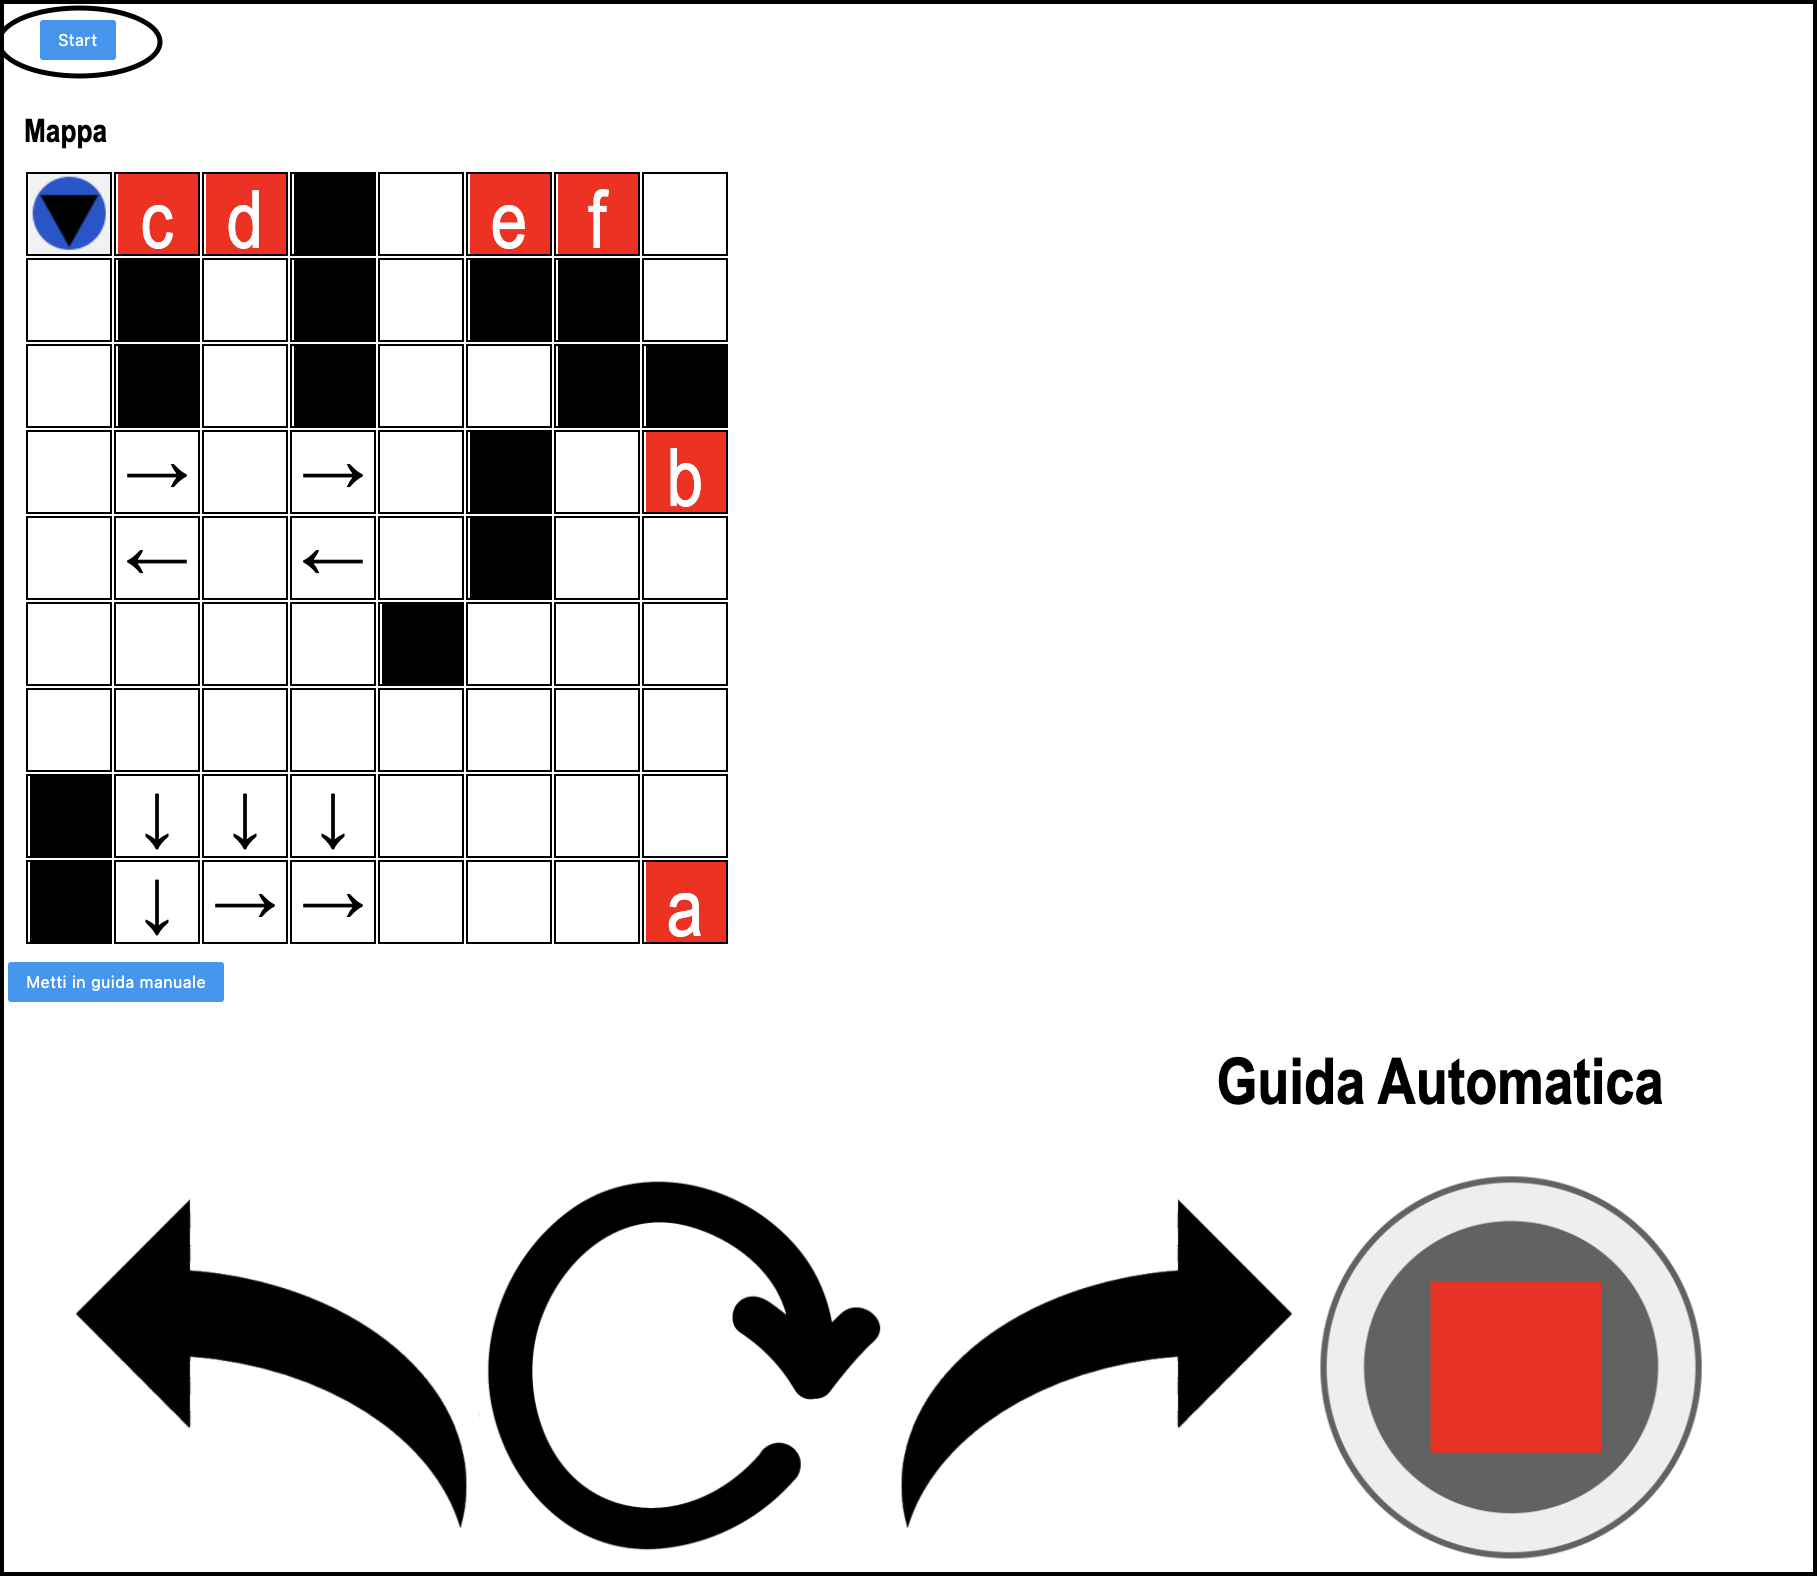
\includegraphics[scale=0.45]{res/images/forklift_start.png}
    \caption{Istantanea dello schermo guida automatica dell'unità}
\end{figure}
\pagebreak
\subsection{Passaggio a guida automatica / guida manuale}
\begin{itemize}
    \item Premere sul pulsante dedicato al cambio di guida "Metti in guida automatica" / "Metti in guida manuale";
    \item i comandi verranno cambiati in base allo stato di guida.
\end{itemize}
\begin{figure}[H]
\centering
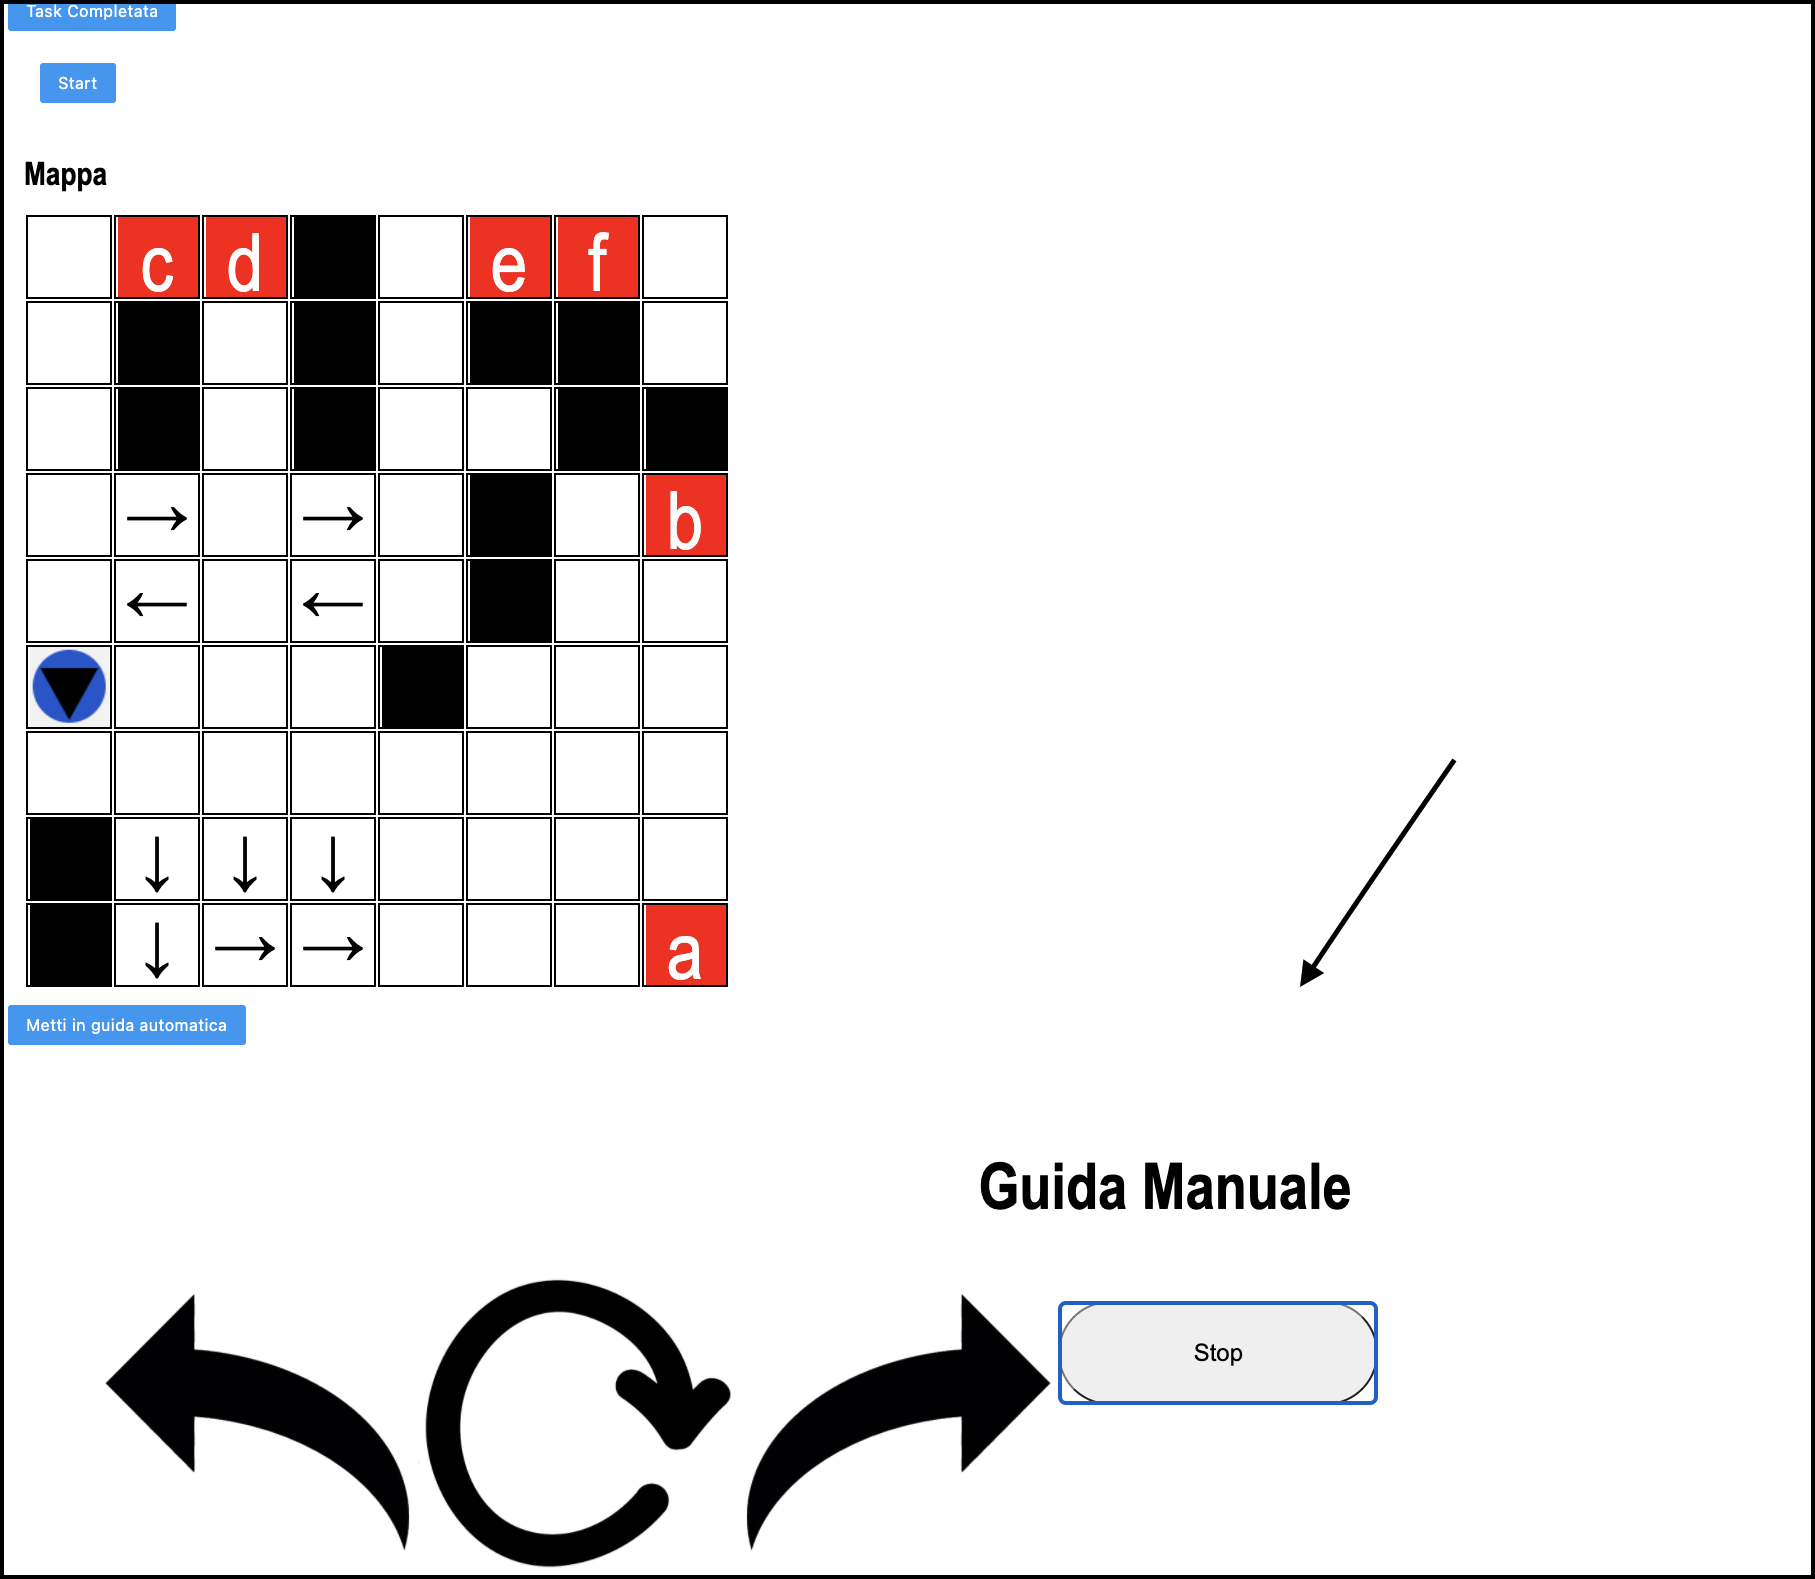
\includegraphics[scale=0.45]{res/images/forklift_guidamanuale.png}
\caption{Istantanea dello schermo passaggio a guida manuale}
\end{figure}

\begin{figure}[H]
    \centering
    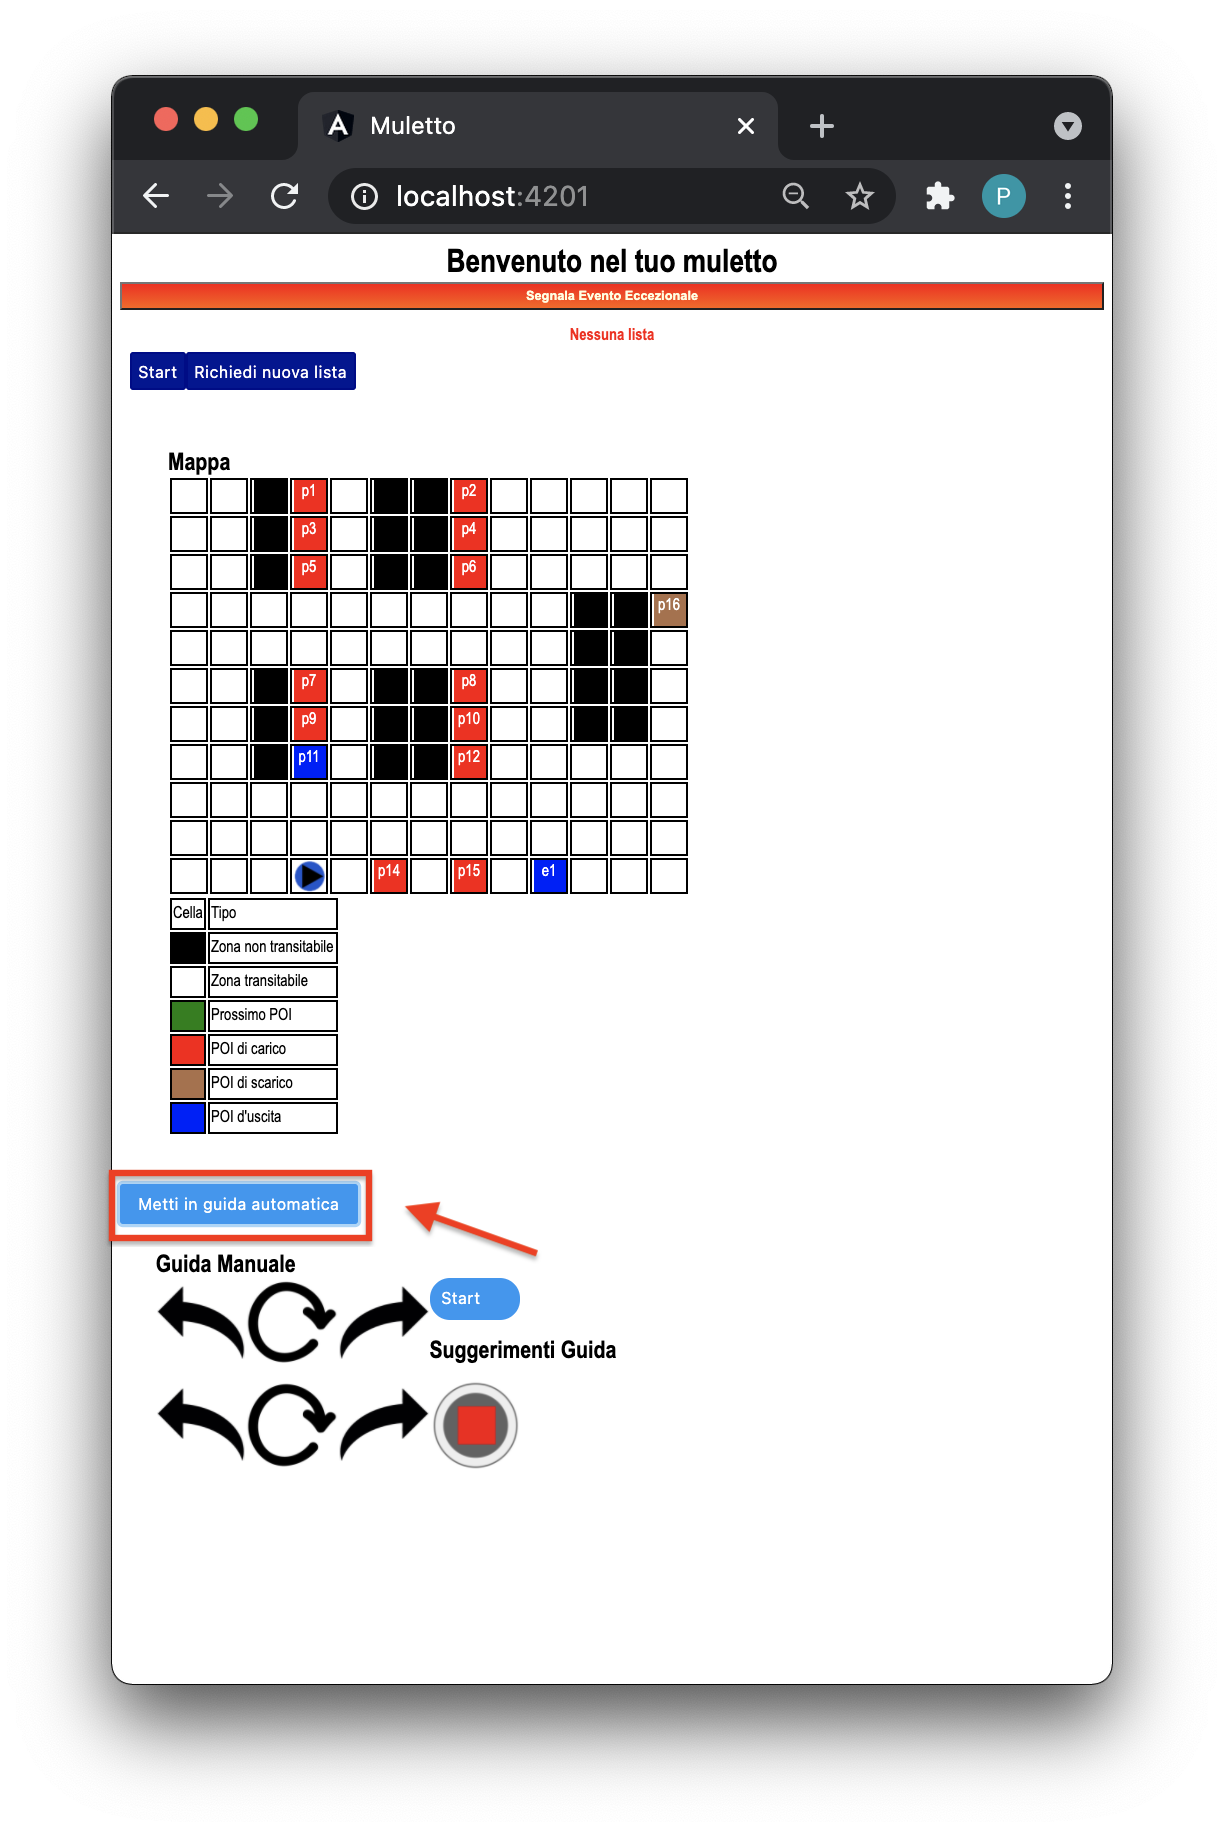
\includegraphics[scale=0.45]{res/images/forklift_cambioautomatica.png}
    \caption{Istantanea dello schermo passaggio a guida automatica}
\end{figure}
\pagebreak

\subsection{Guida manuale dell'unità}
\begin{itemize}
    \item Premere sul pulsante "Metti in guida manuale";
    \begin{figure}[H]
        \centering
          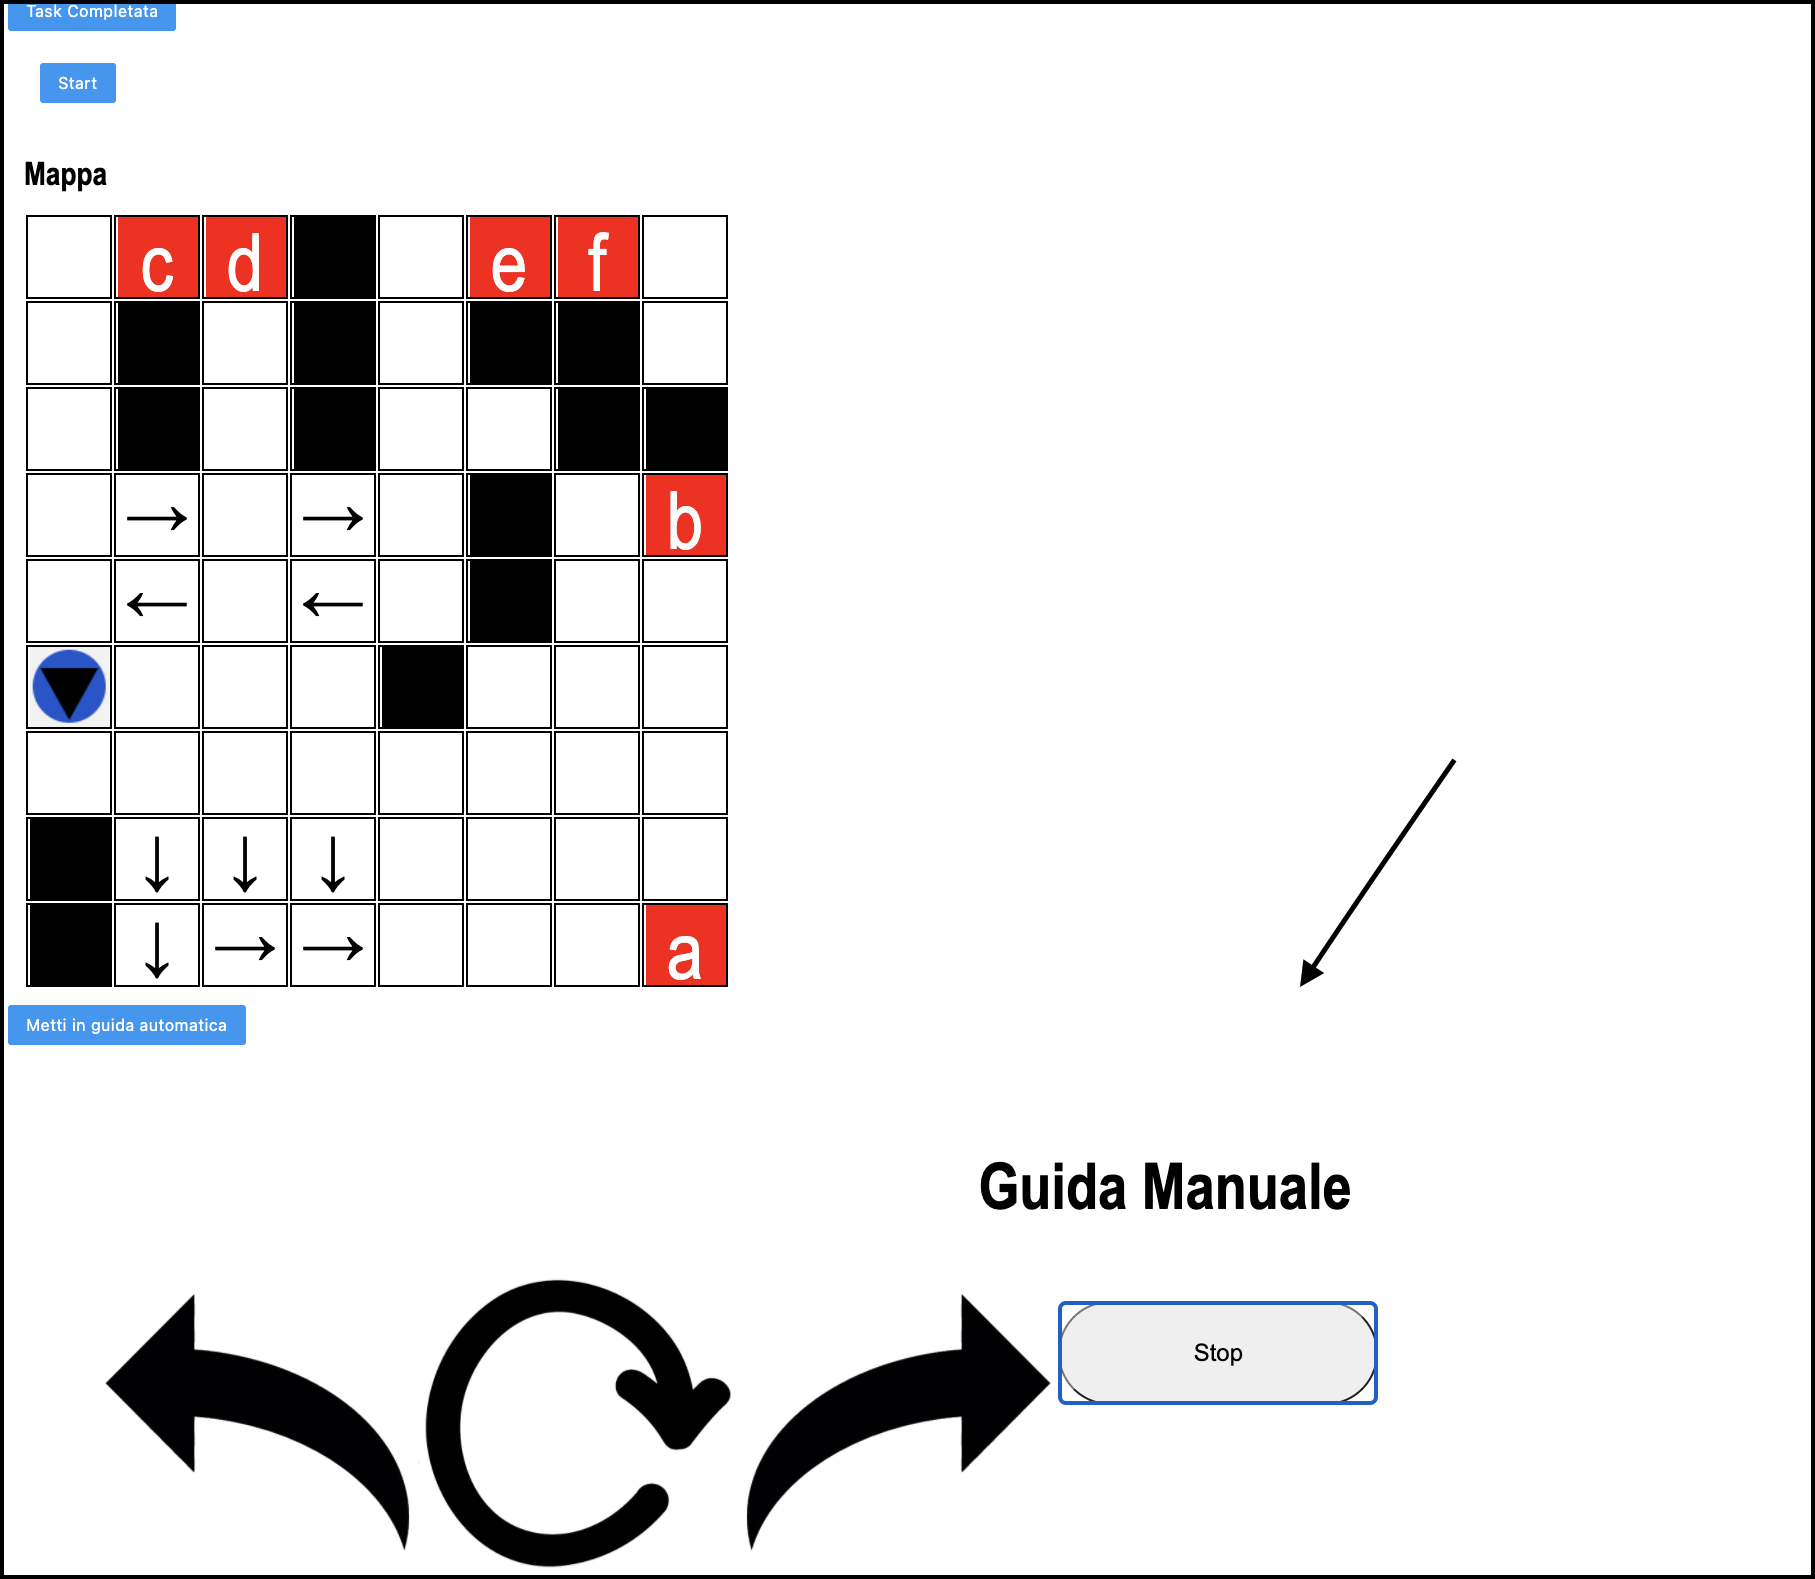
\includegraphics[scale=0.45]{res/images/forklift_guidamanuale.png}
          \caption{Istantanea dello schermo guida manuale dell'unità - pulsante cambio guida}
    \end{figure}
    \item tramite il pulsante "Start" viene avviato il movimento del muletto verso la direzione in cui è rivolto;
    \begin{figure}[H]
        \centering
          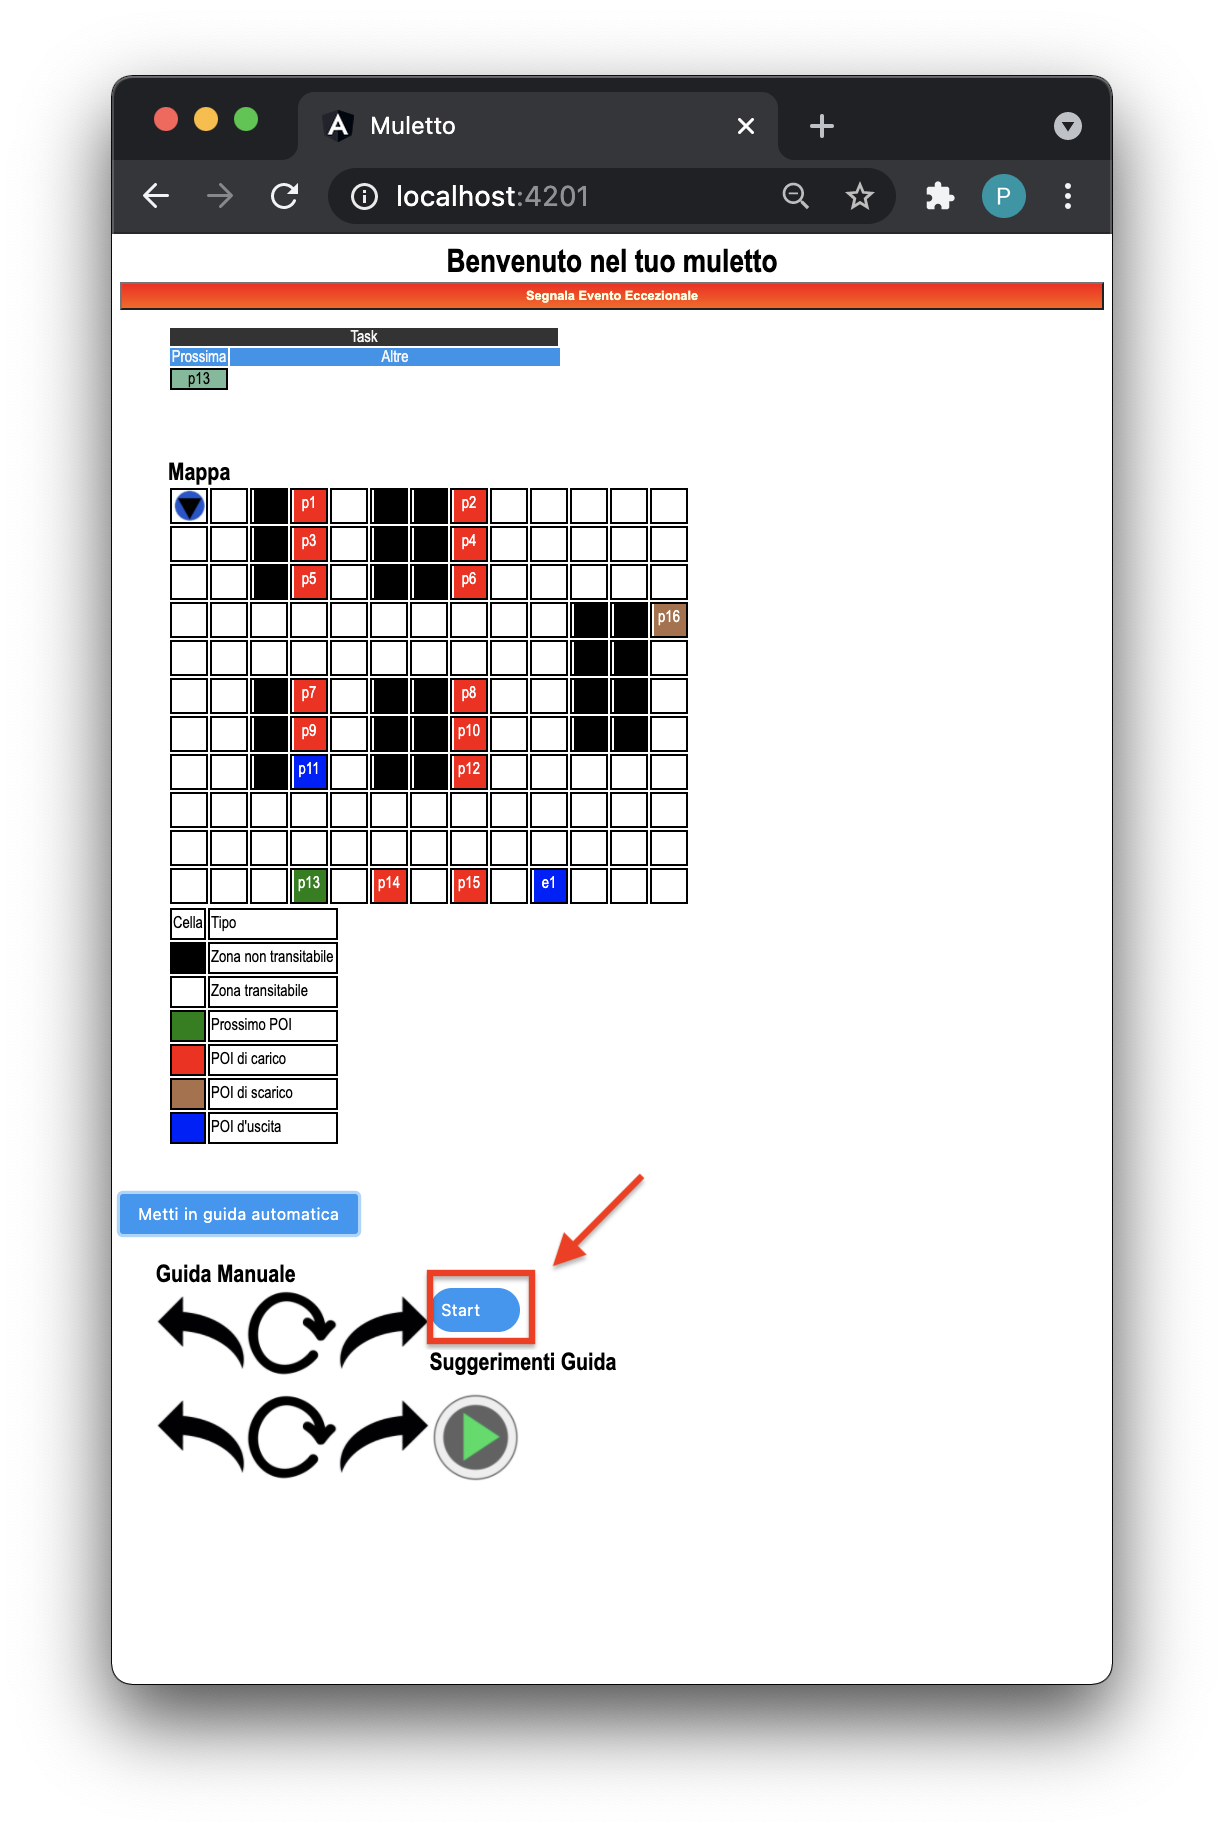
\includegraphics[scale=0.45]{res/images/guidamanuale.png}
          \caption{Istantanea dello schermo guida manuale dell'unità - pulsante start}
    \end{figure}
    \item premendo le frecce il muletto ruota di 90 o di 180 gradi;
    \begin{figure}[H]
        \centering
          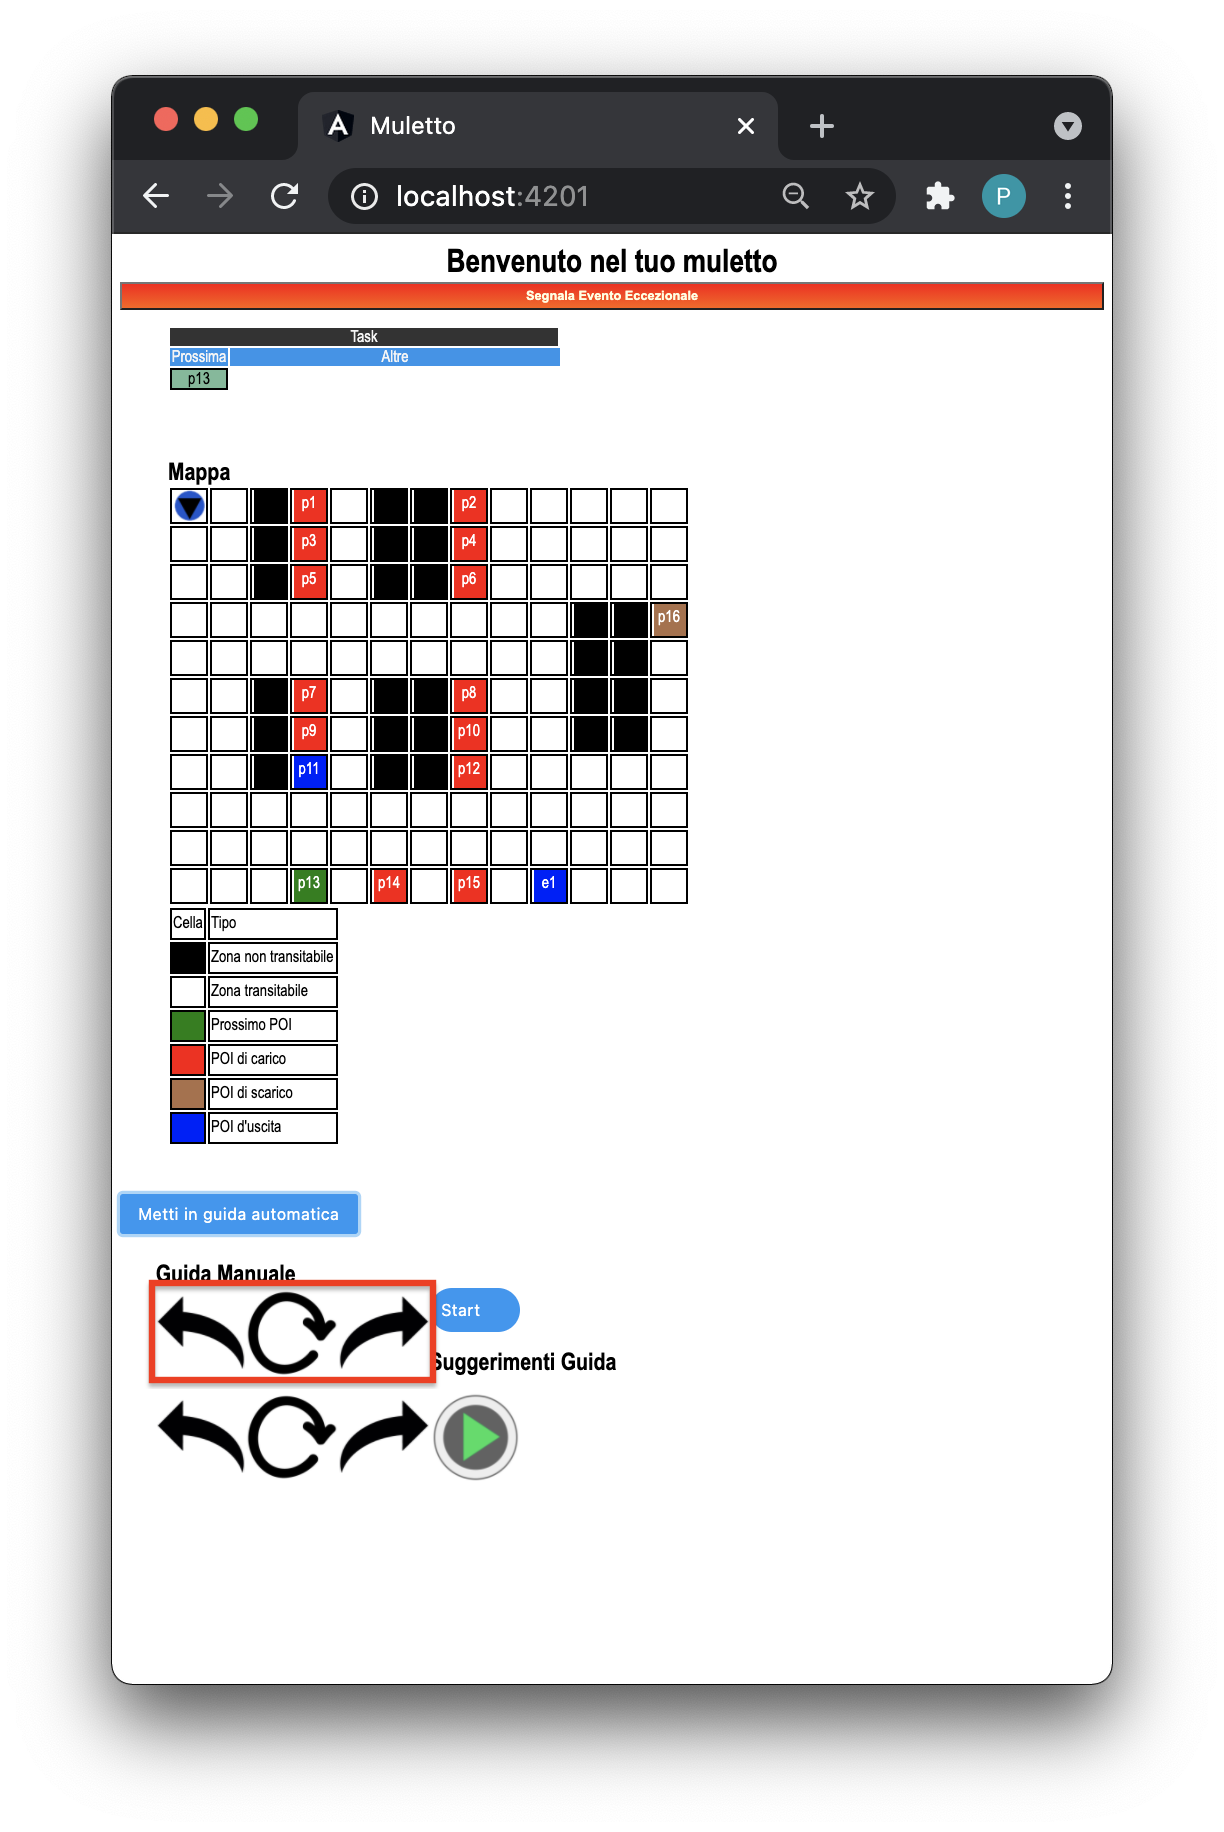
\includegraphics[scale=0.45]{res/images/guidamanuale1.png}
          \caption{Istantanea dello schermo guida manuale dell'unità - pulsanti di rotazione dell'unità}
    \end{figure}
    \item premendo il pulsante "Stop" viene fermato il movimento;
    \begin{figure}[H]
        \centering
          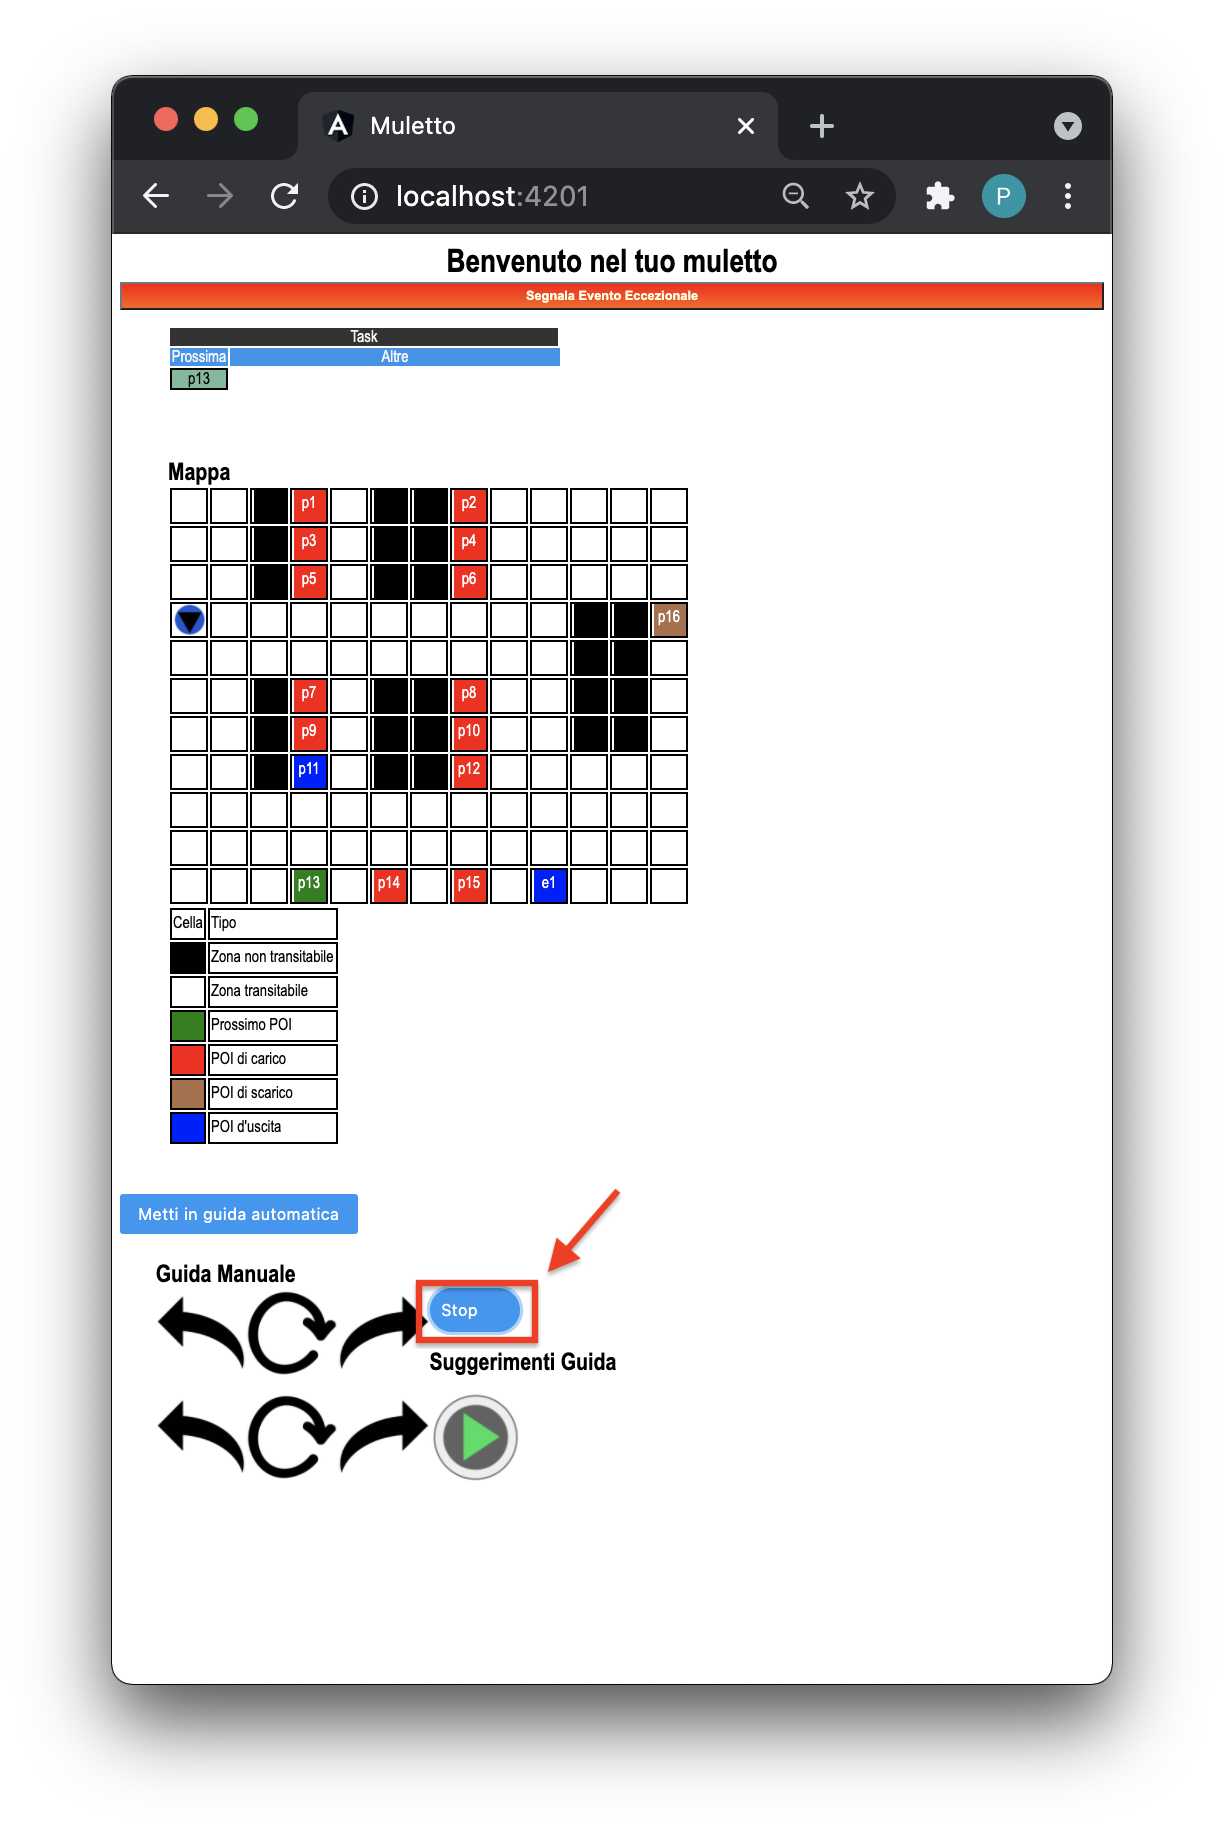
\includegraphics[scale=0.45]{res/images/guidamanuale_stop.png}
          \caption{Istantanea dello schermo guida manuale dell'unità - pulsante stop}
    \end{figure}
    \item sotto sono visualizzati i suggerimenti dei pulsanti da premere per il raggiungimento del POI interessato nel più breve percorso possibile.
    \begin{figure}[H]
        \centering
          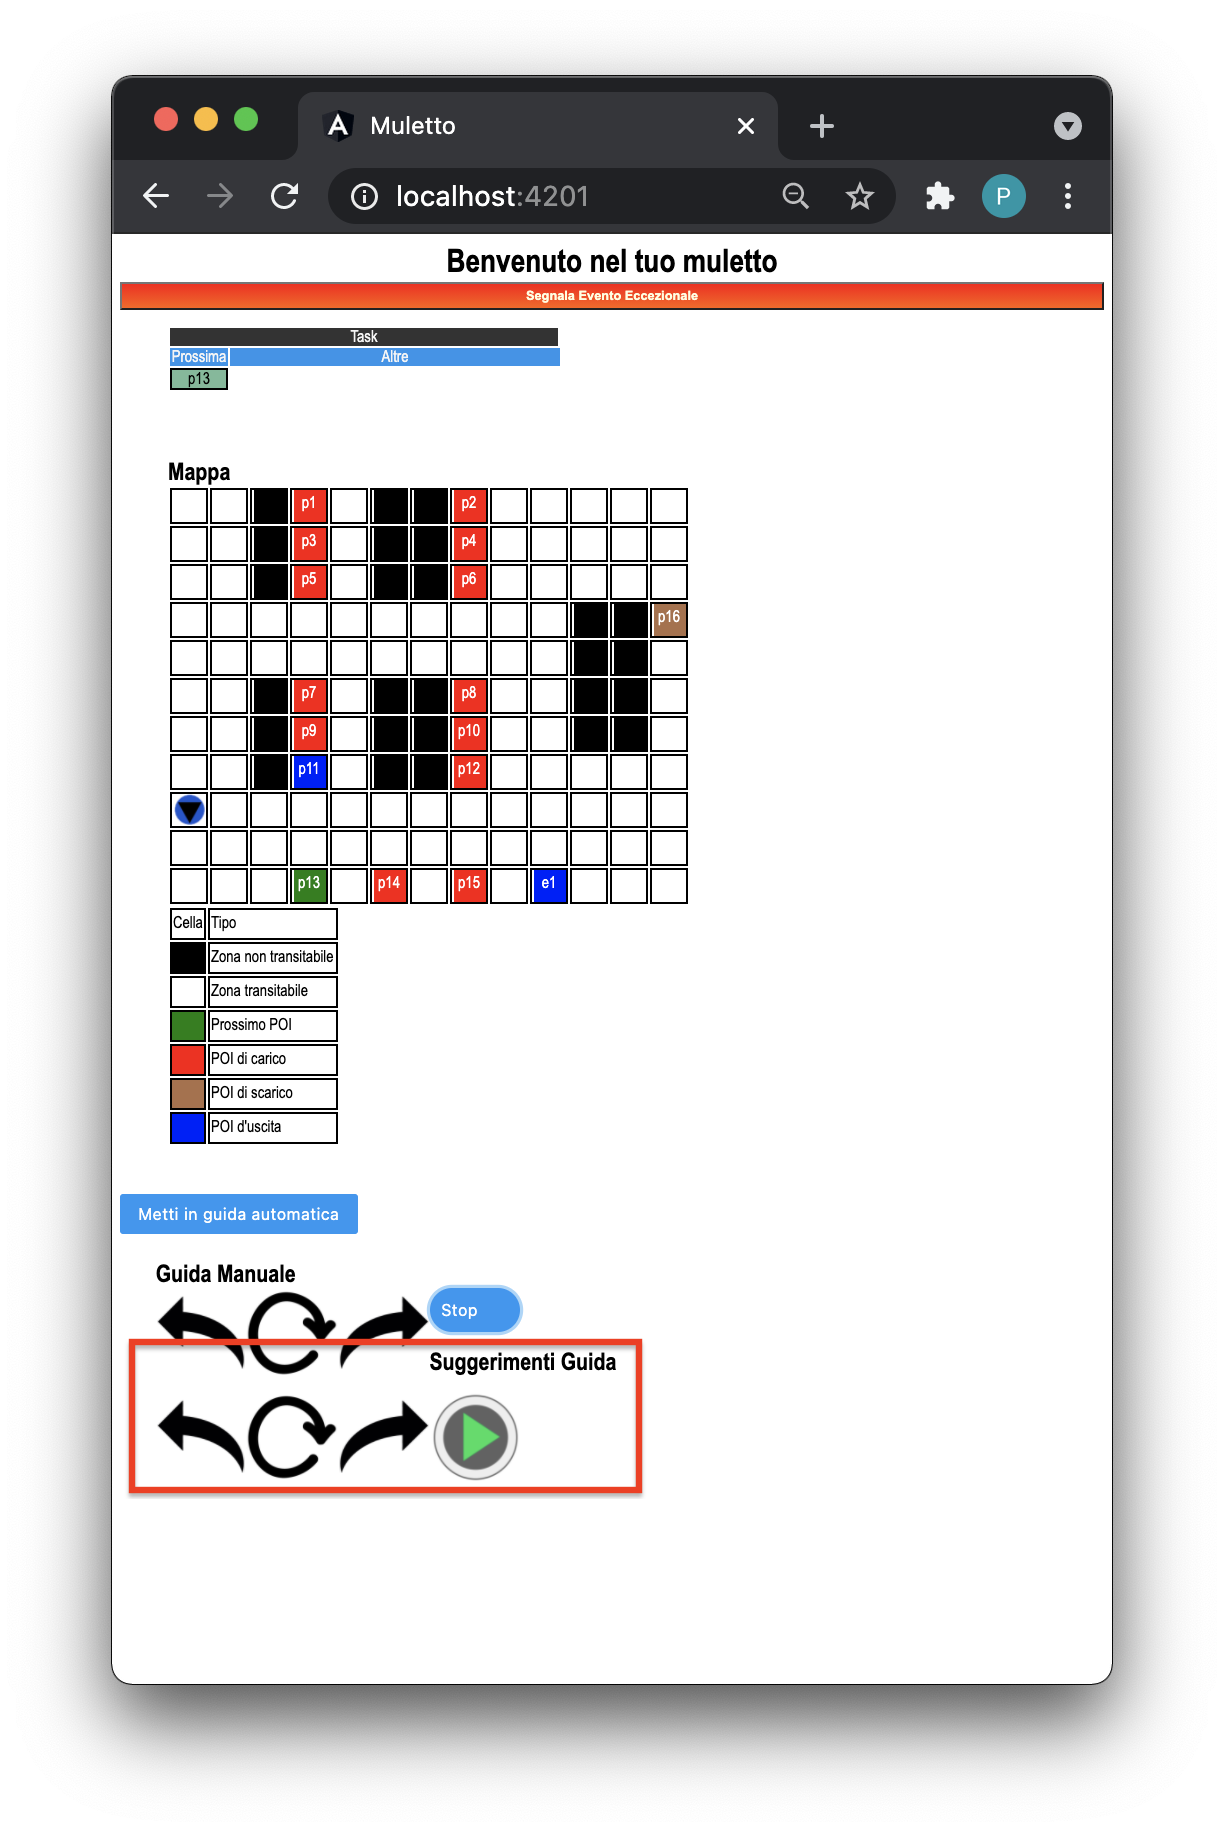
\includegraphics[scale=0.45]{res/images/suggerimenti.png}
          \caption{Istantanea dello schermo guida manuale dell'unità - suggerimenti di guida}
    \end{figure}
\end{itemize}

\subsection{Completamento task}
\begin{itemize}
    \item Una volta raggiunto il POI, l'unità si ferma in caso di guida automatica e viene visualizzato il pulsante "Task completata";
    \item premere il pulsante per notificare la fine dell'azione (in relazione al tipo di POI) e per passare al prossimo POI, col relativo movimento dell'unità in caso di guida automatica;
    \begin{figure}[H]
        \centering
        	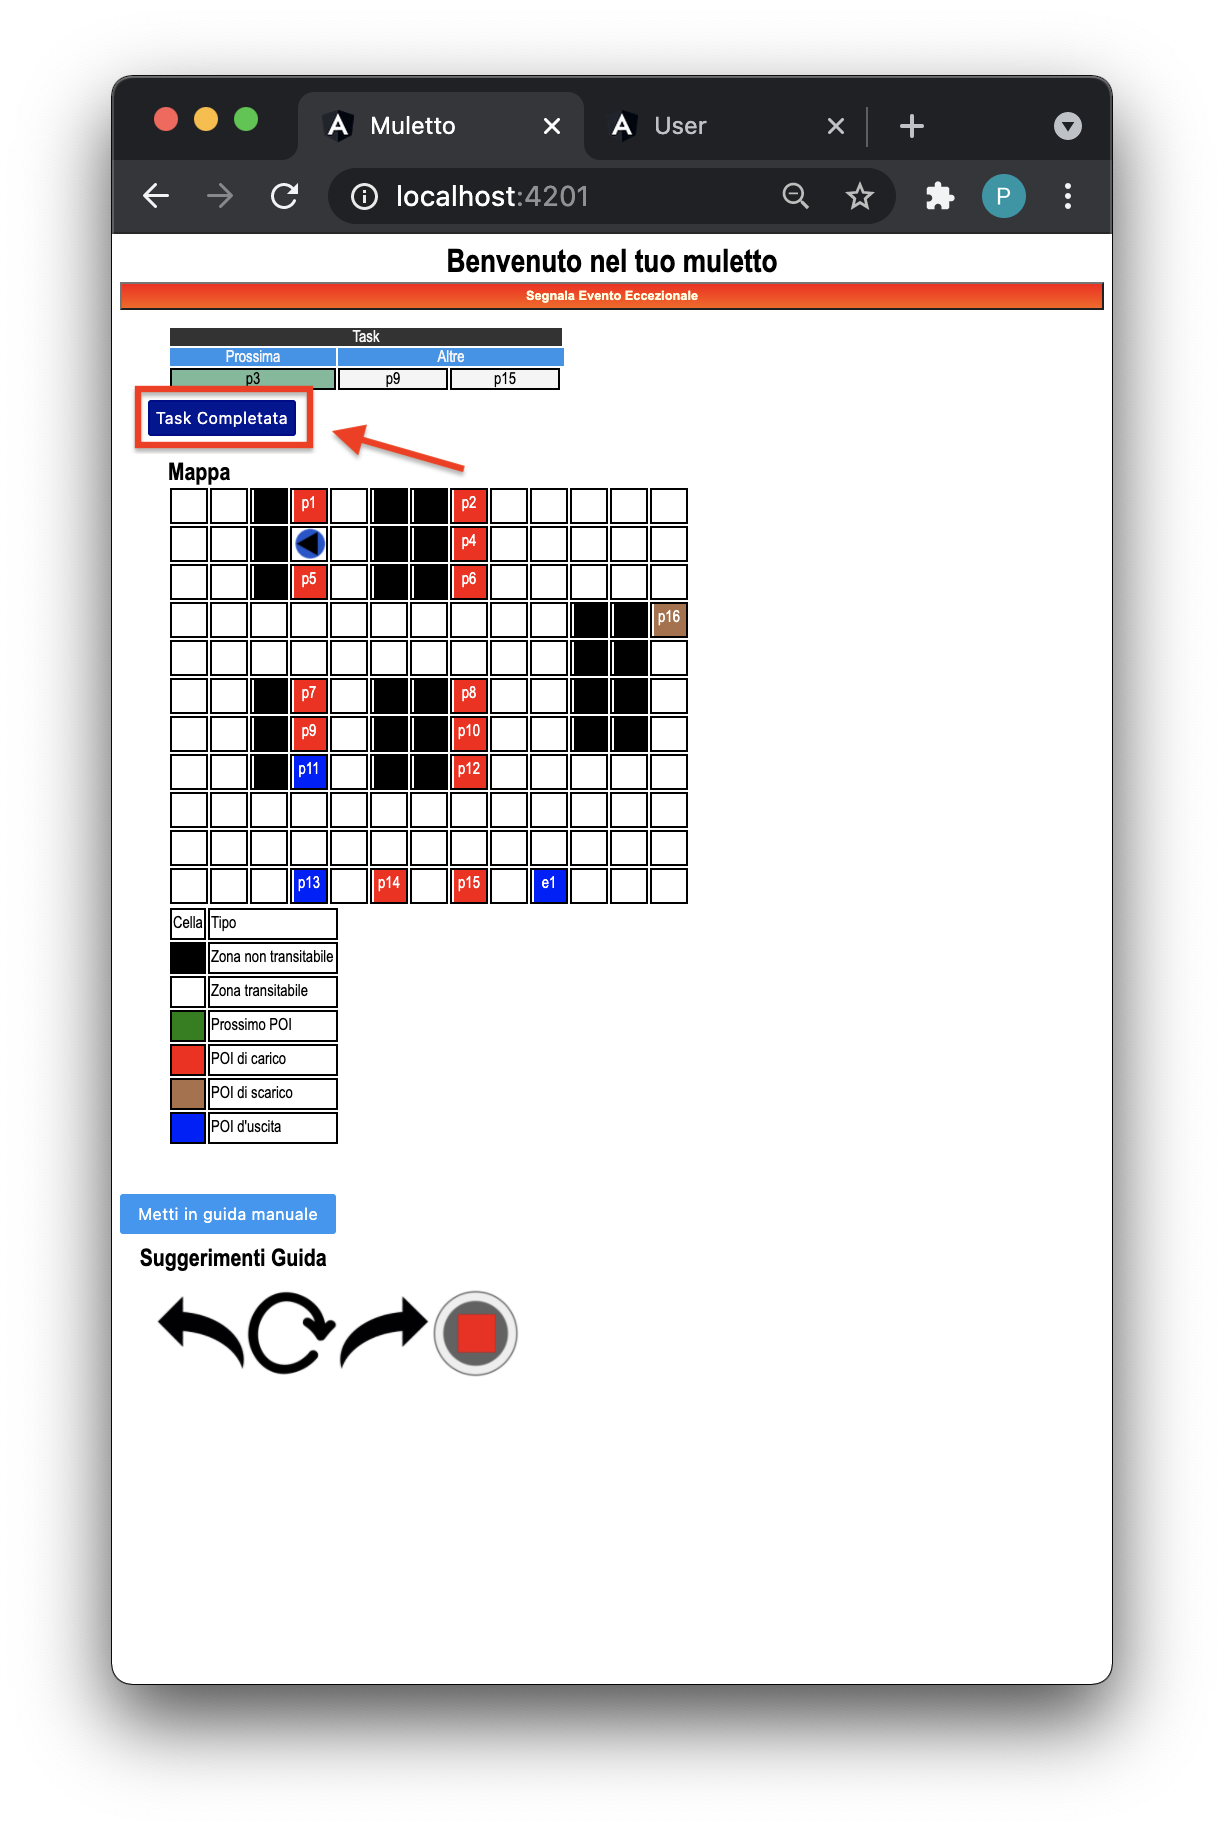
\includegraphics[scale=0.45]{res/images/forklift_taskcompletata.png}
        	\caption{Istantanea dello schermo pulsante task completata}
    \end{figure}
    \item verrà quindi evidenziato in verde il prossimo POI da raggiungere.
    \begin{figure}[H]
        \centering
        	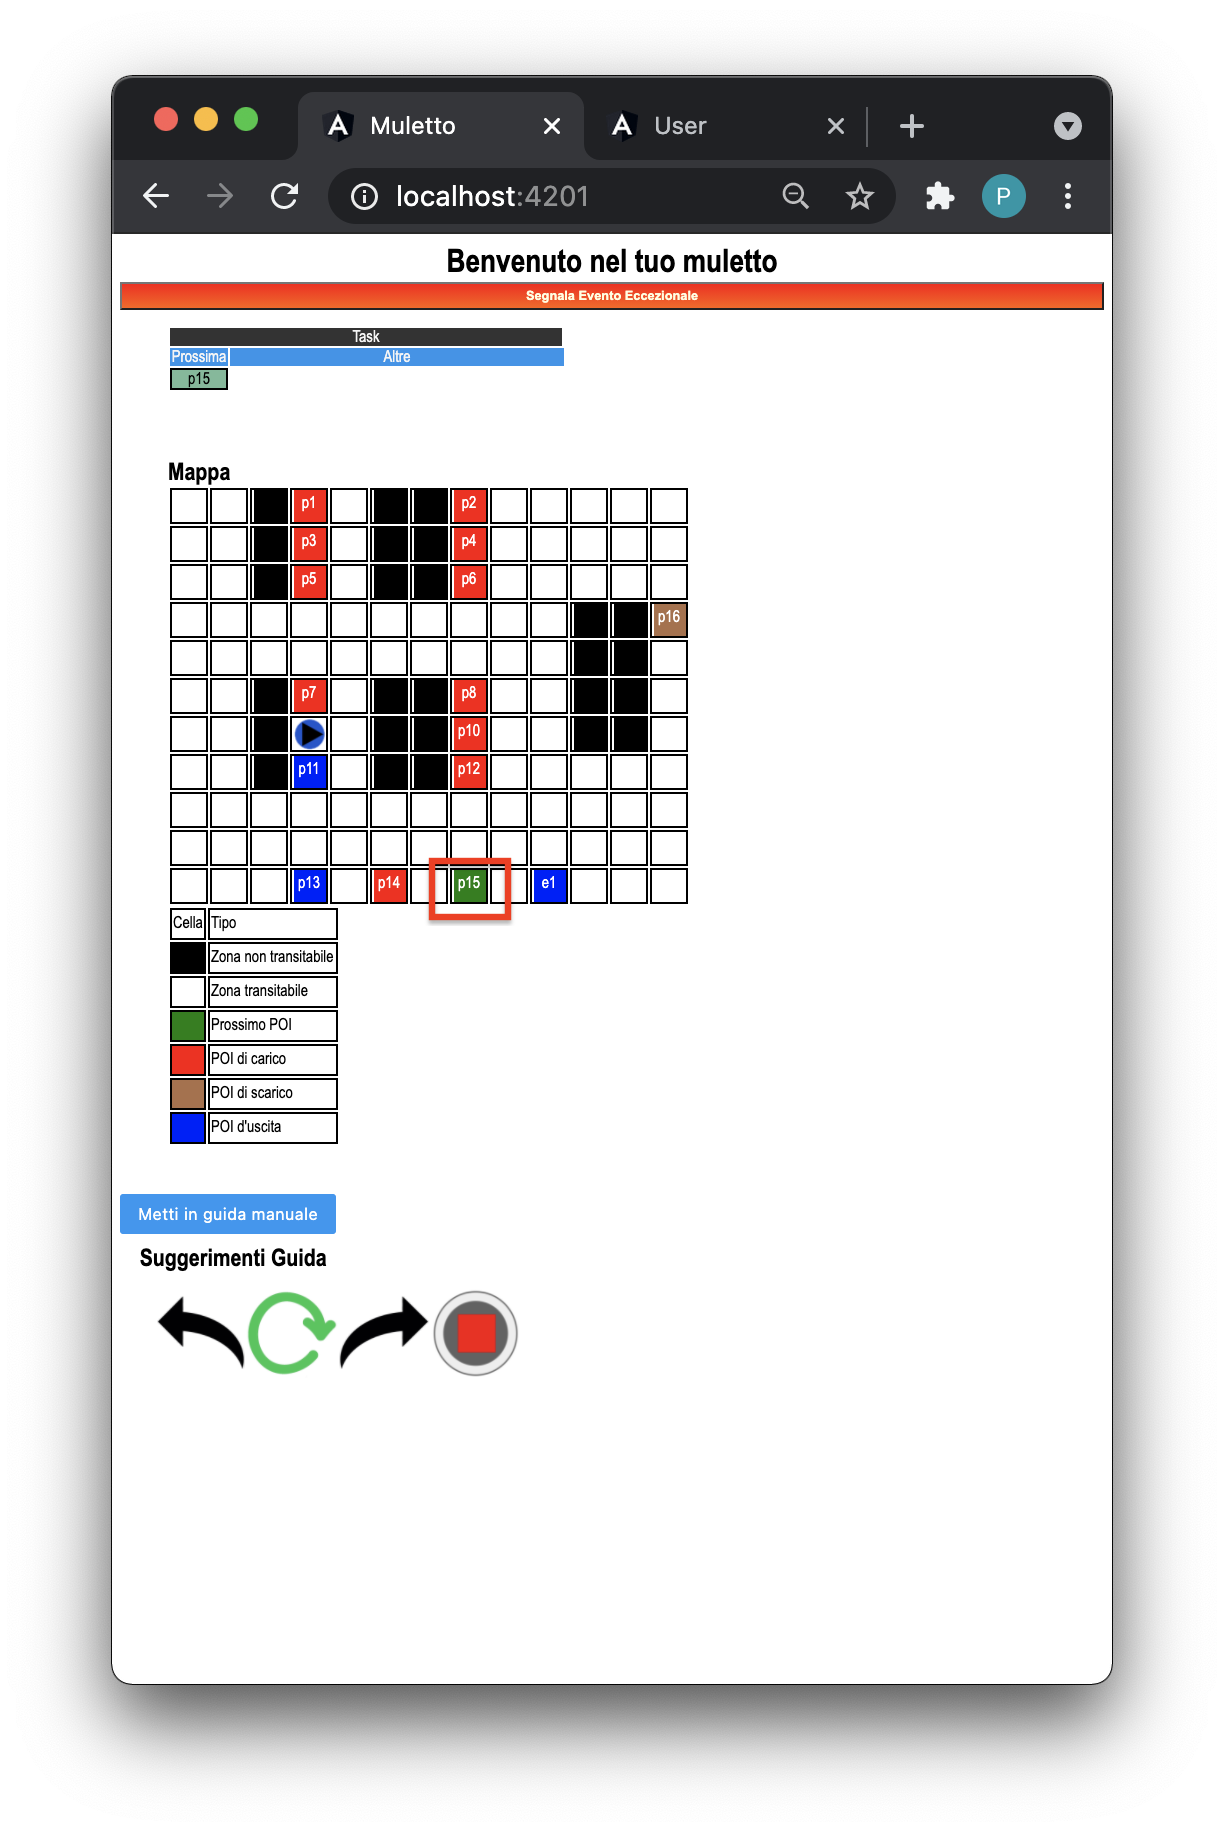
\includegraphics[scale=0.45]{res/images/next.png}
        	\caption{Istantanea dello schermo prossimo POI evidenziato col colore verde}
    \end{figure}
\end{itemize}
\subsection{Ritorno alla base}
\begin{itemize}
    \item Quando sono finite le liste di task disponibili, viene visualizzata la base più vicina da raggiungere.
    \item premere il pulsante "Start" per recarsi in essa.
\end{itemize}
\begin{figure}[H]
    \centering
    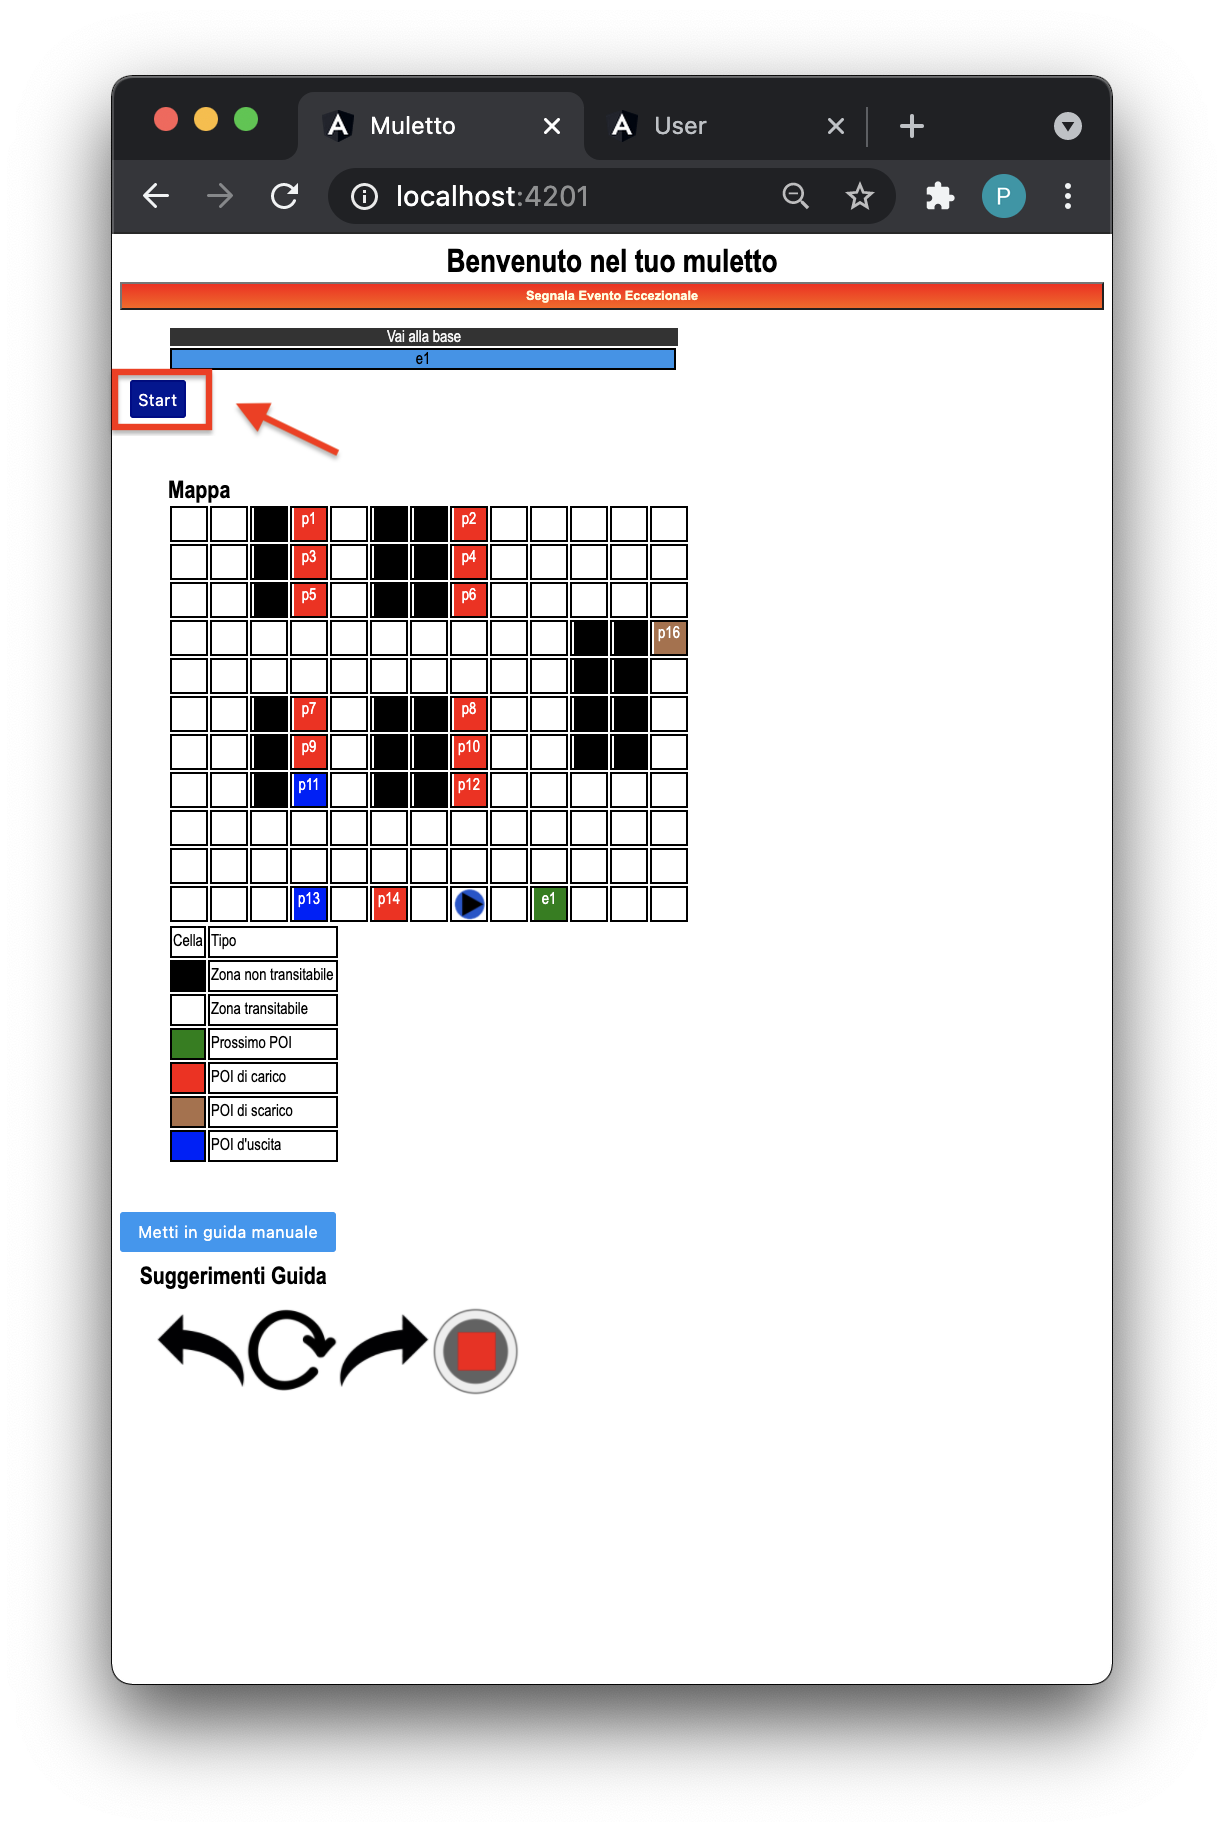
\includegraphics[scale=0.45]{res/images/ritornoallabase.png}
    \caption{Istantanea dello schermo ritorno alla base}
\end{figure}

\subsection{Richiesta nuova lista di task}
\begin{itemize}
    \item Quando ci si trova in base è possibile richiedere una nuova lista di task premendo su "Richiedi nuova lista"
    \begin{figure}[H]
        \centering
        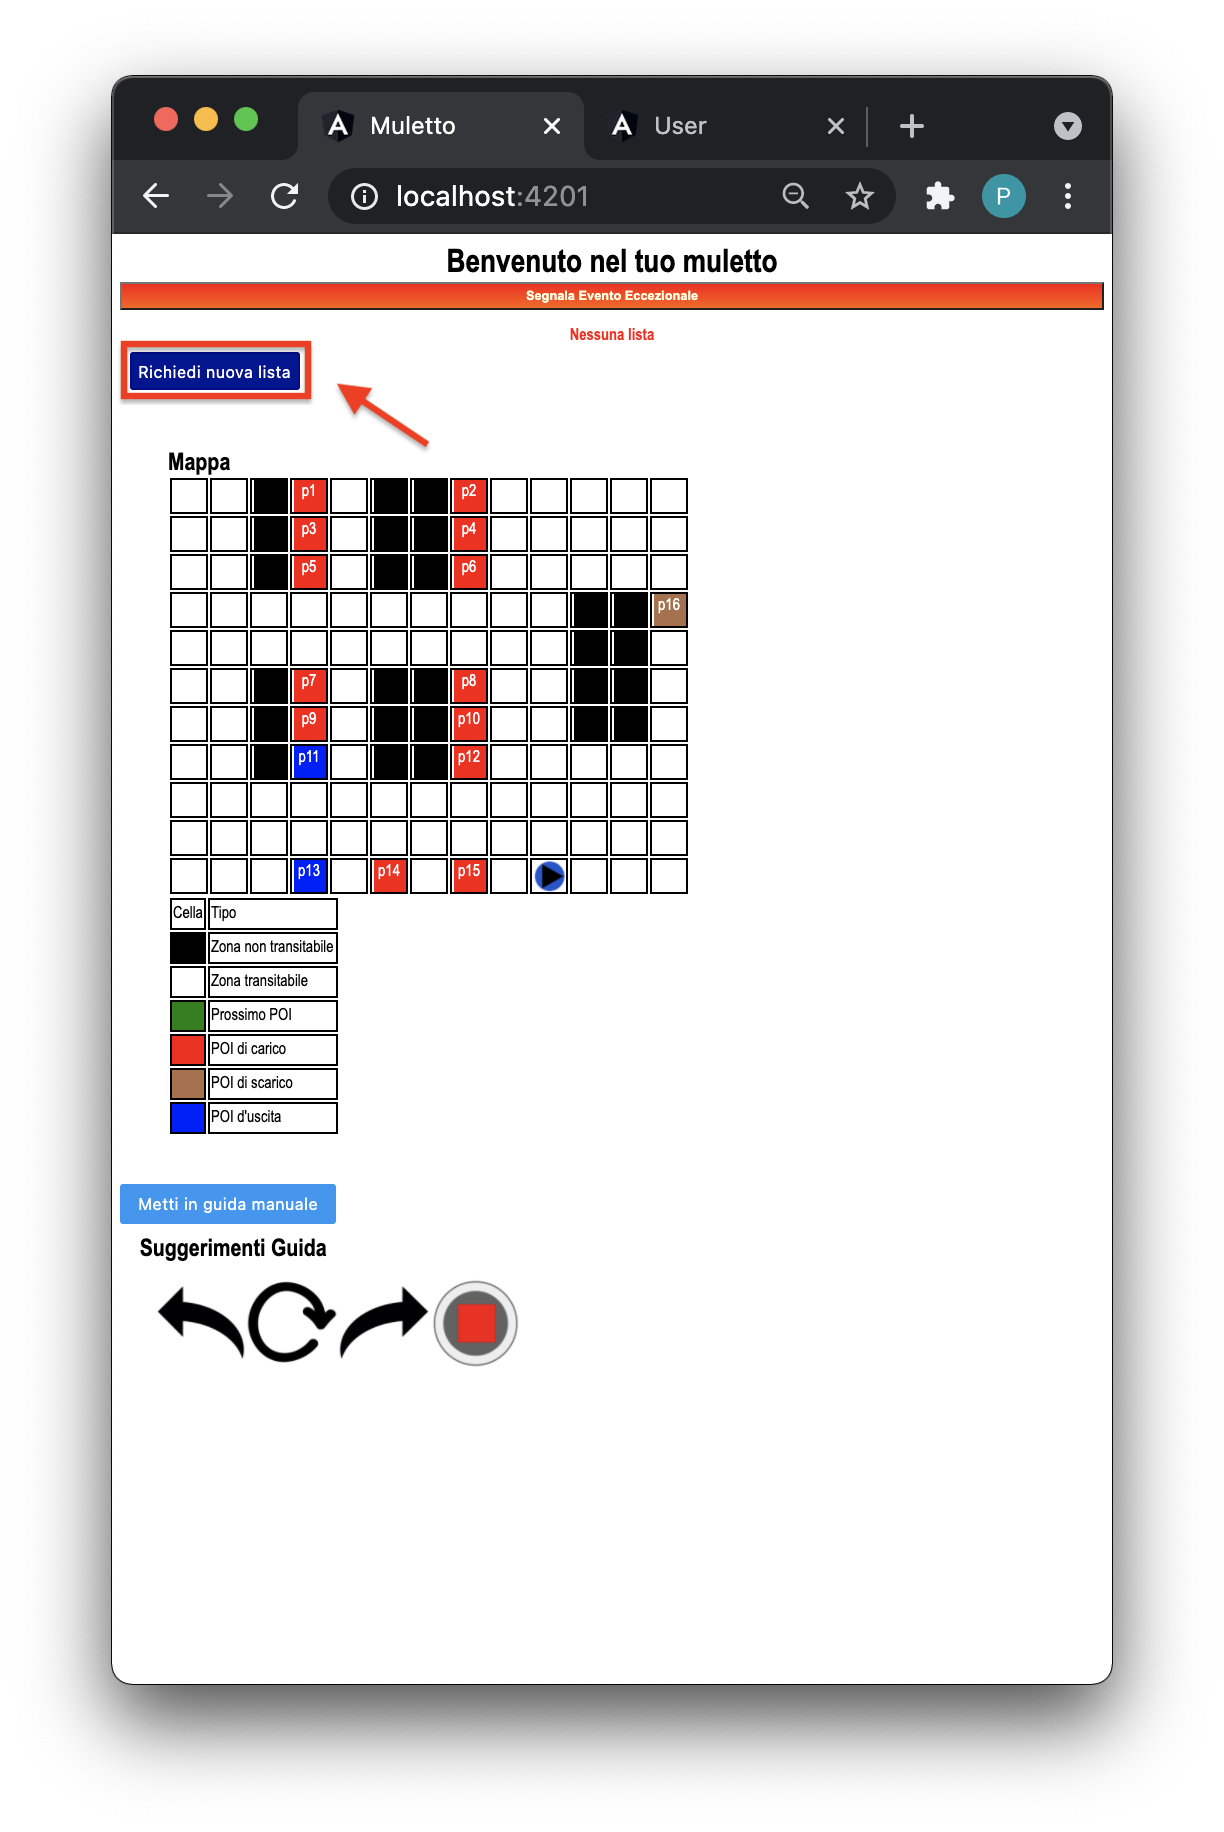
\includegraphics[scale=0.45]{res/images/nuovalista.png}
        \caption{Istantanea dello schermo richiesta nuova lista}
    \end{figure}
    \item se non è presente alcuna lista disponibile bisognerà riprovare più tardi.
    \begin{figure}[H]
        \centering
        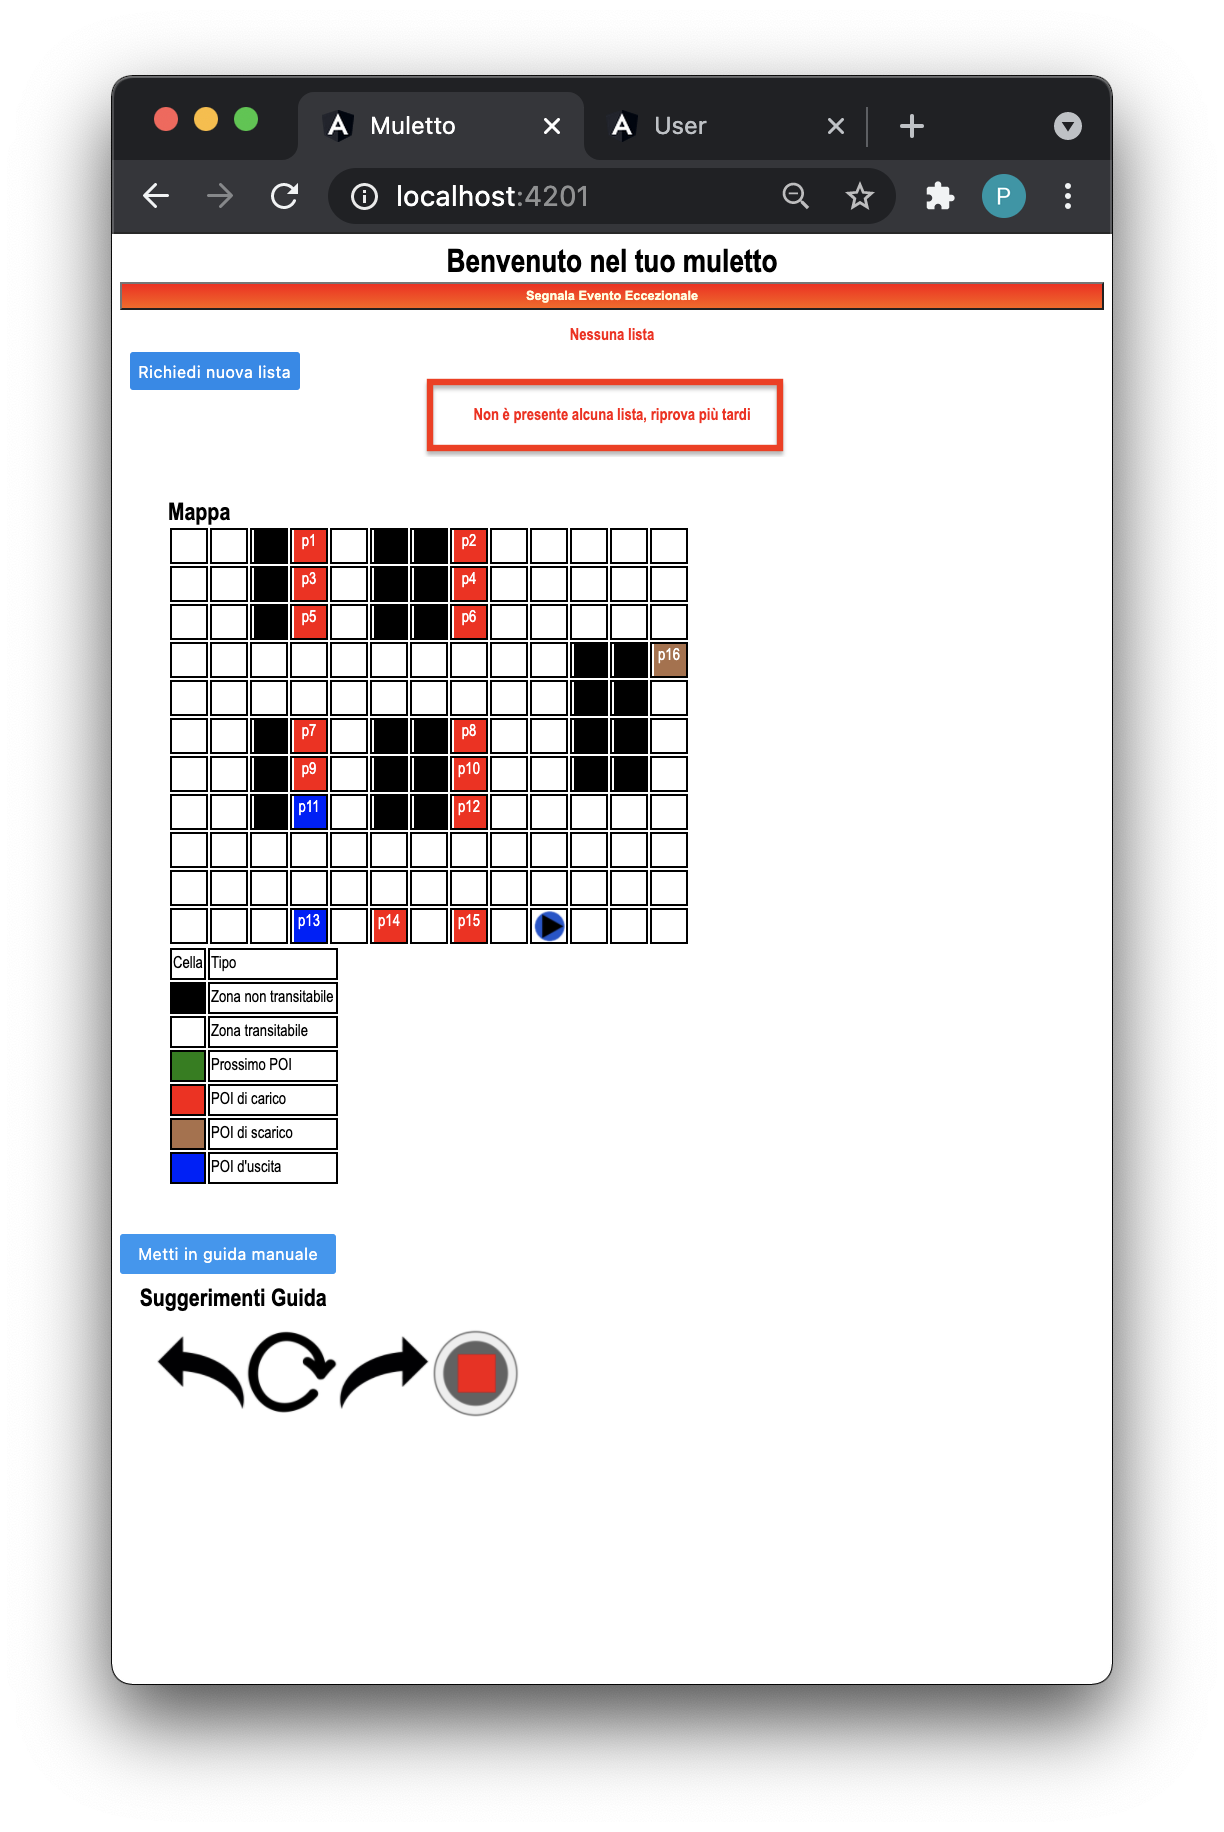
\includegraphics[scale=0.45]{res/images/nolist.png}
        \caption{Istantanea dello schermo nessuna lista disponibile}
    \end{figure}
\end{itemize}



\subsection{Segnalazione evento eccezionale}
\begin{itemize}
    \item Premere sul pulsante "Evento eccezionale" per notificare all'amministratore l'avvenimento di un evento non previsto.
\end{itemize}
\begin{figure}[H]
    \centering
    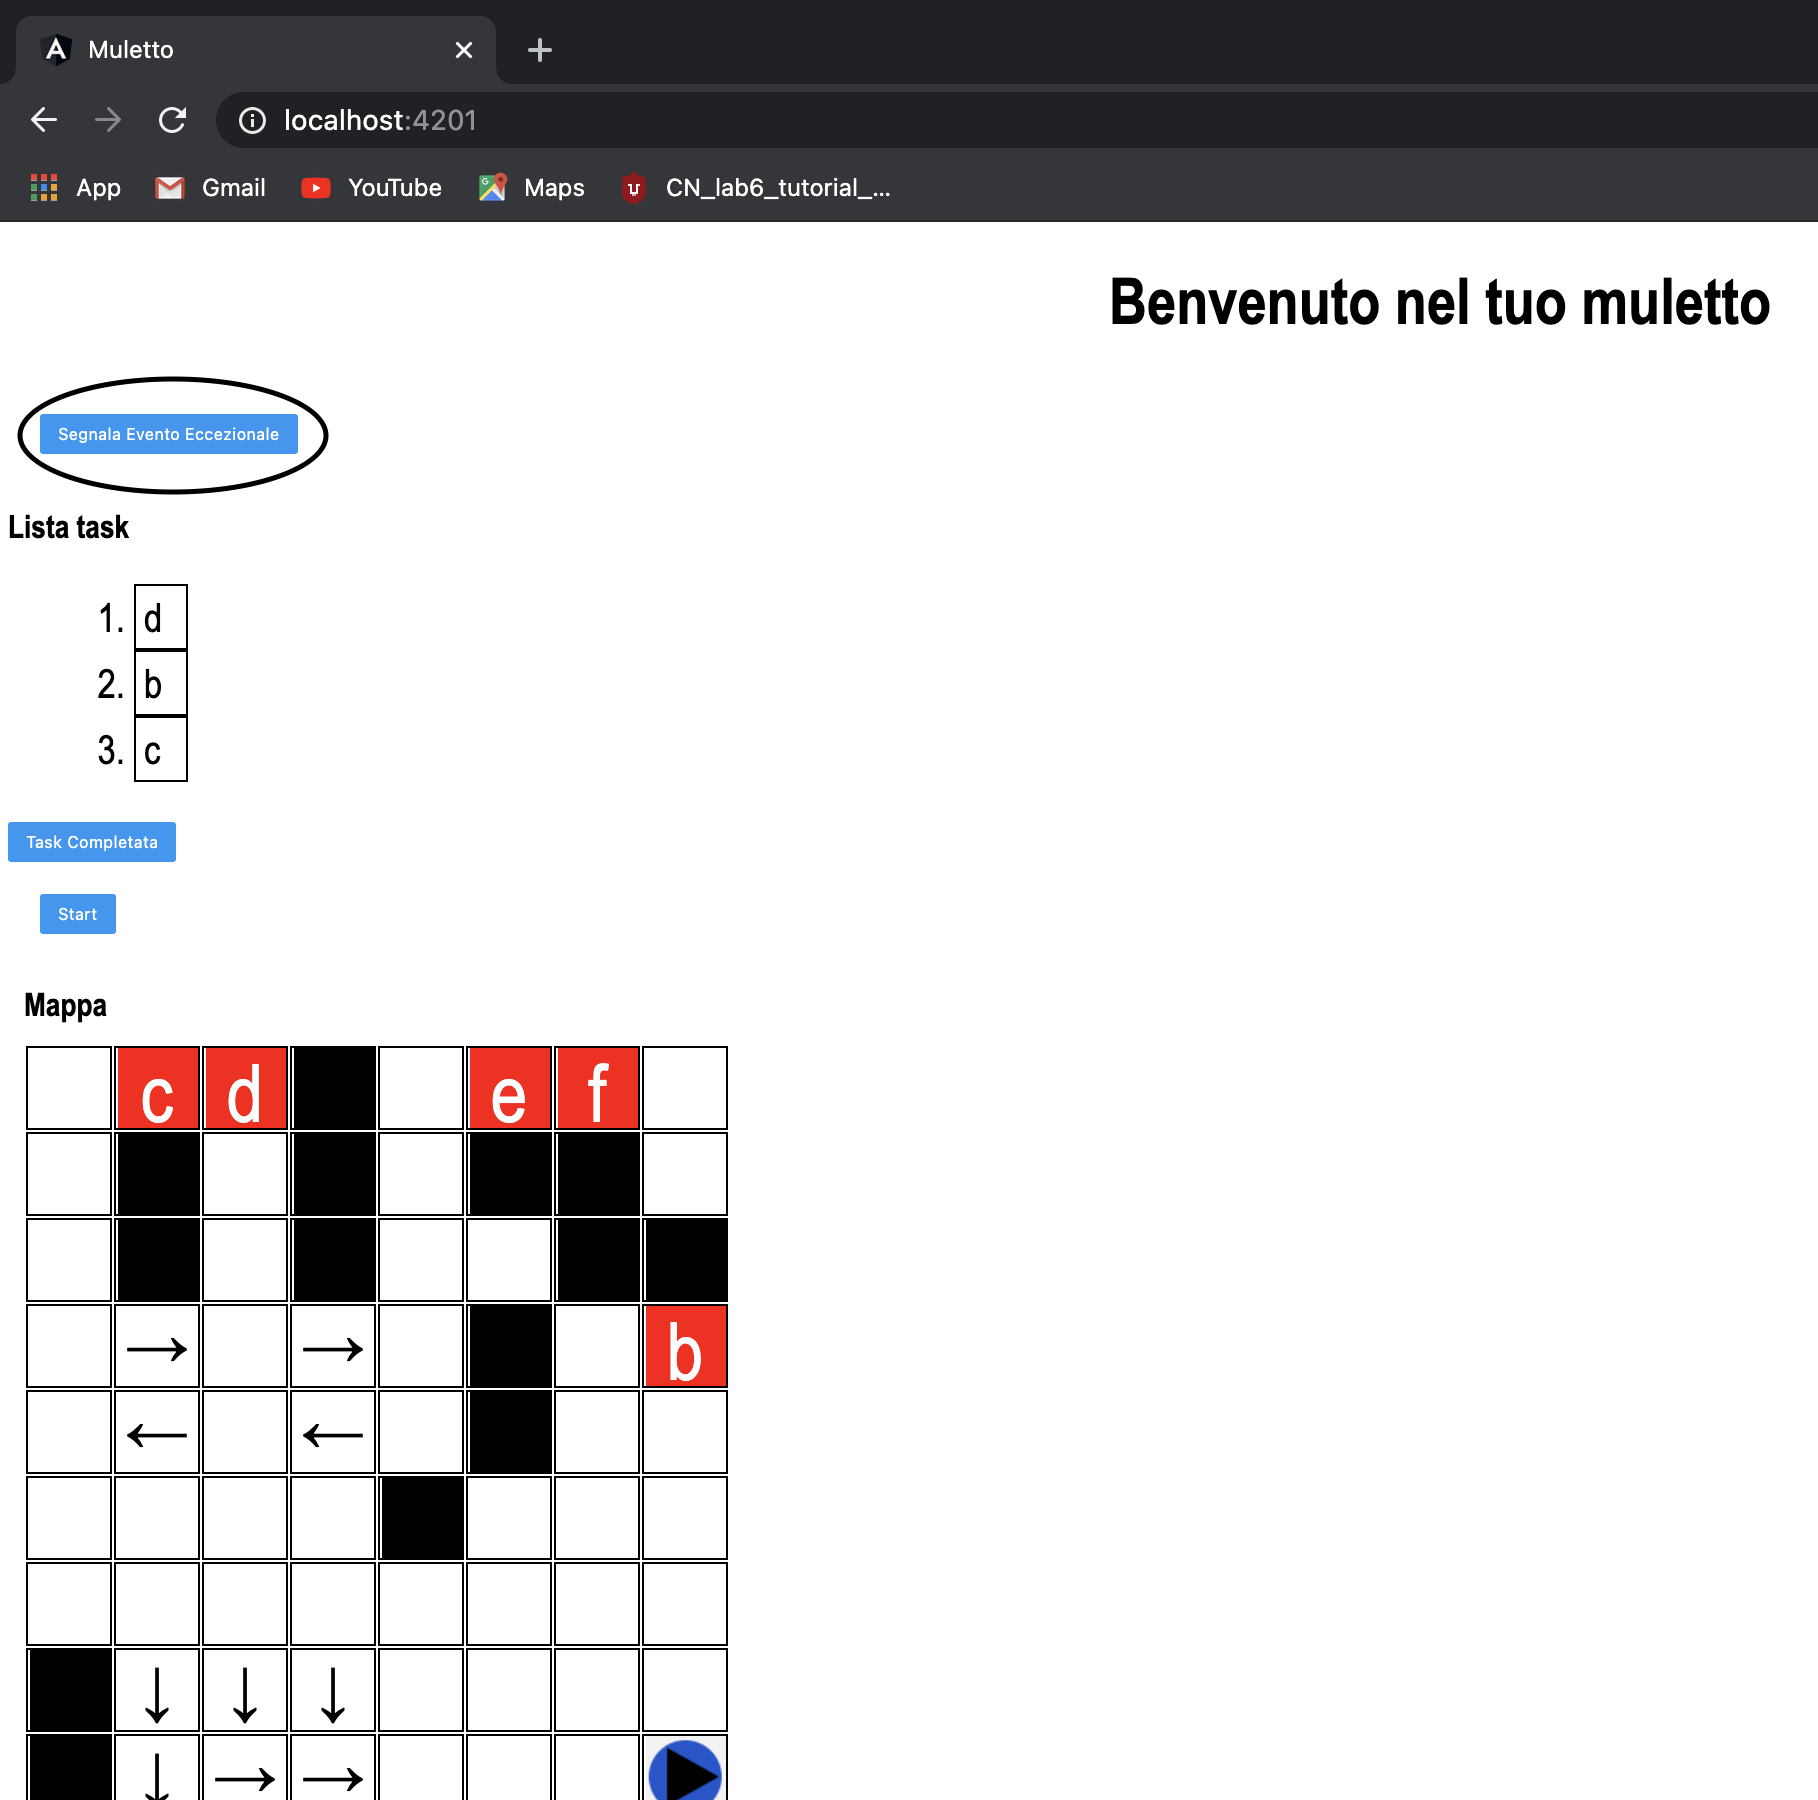
\includegraphics[scale=0.45]{res/images/forklift_evento.png}
    \caption{Istantanea dello schermo segnalazione evento eccezionale}
\end{figure}